\documentclass[11pt,a4paper]{article}

% ============================================================================
% PAQUETES
% ============================================================================
\usepackage[utf8]{inputenc}
\usepackage[spanish]{babel}
\usepackage[T1]{fontenc}
\usepackage{amsmath,amsfonts,amssymb}
\usepackage{graphicx}
\usepackage{booktabs}
\usepackage{float}
\usepackage{hyperref}
\usepackage{geometry}
\usepackage{setspace}
\usepackage{natbib}
\usepackage{caption}
\usepackage{subcaption}
\usepackage{multirow}
\usepackage{array}
\usepackage{xcolor}
\usepackage{fancyhdr}
\usepackage{longtable}
\usepackage{pdflscape}
\usepackage{titlesec}
\usepackage{enumitem}

% Configuracion de pagina
\geometry{margin=2.5cm, headheight=14pt}
\setstretch{1.5}

% Configuracion de encabezados
\pagestyle{fancy}
\fancyhf{}
\fancyhead[L]{\small\textit{Deep Learning y Triple Screen de Elder para Predicción del S\&P 500}}
\fancyhead[R]{\small\thepage}
\renewcommand{\headrulewidth}{0.4pt}

% Configuracion de hyperref
\hypersetup{
    colorlinks=true,
    linkcolor=blue!70!black,
    filecolor=magenta,
    urlcolor=cyan!70!black,
    citecolor=blue!70!black
}

% Formato de secciones
\titleformat{\section}{\large\bfseries}{\thesection.}{0.5em}{}
\titleformat{\subsection}{\normalsize\bfseries}{\thesubsection}{0.5em}{}
\titleformat{\subsubsection}{\normalsize\itshape}{\thesubsubsection}{0.5em}{}

% ============================================================================
% DOCUMENTO
% ============================================================================
\begin{document}

% ============================================================================
% TITULO
% ============================================================================
\thispagestyle{empty}
\begin{center}

\vspace*{0.8cm}

{\LARGE\bfseries Desafiando la Eficiencia del Mercado:\par}
\vspace{0.5cm}
{\Large\bfseries Aprendizaje Profundo y el Sistema Triple Screen de Elder\\ para la Predicción de Retornos del S\&P 500\par}

\vspace{1.2cm}

{\large David González Canón\par}
\vspace{0.4cm}
{\normalsize Maestría en Inteligencia de Negocios para Finanzas\par}
\vspace{0.2cm}
{\normalsize Diciembre 2025\par}

\vspace{1.2cm}

\noindent\rule{0.9\textwidth}{0.5pt}

\vspace{0.8cm}

\end{center}

\begin{minipage}{0.95\textwidth}
\small
\setstretch{1.25}
\textbf{Resumen}

\vspace{0.3cm}

Este estudio investiga si la generación sistemática de alfa es alcanzable mediante la integración del sistema de trading Triple Screen de Alexander Elder con arquitecturas de aprendizaje profundo de última generación. Utilizando un conjunto exhaustivo de 92 variables macroeconómicas, financieras y de sentimiento provenientes de Bloomberg Terminal, construimos 647 características predictivas que incorporan estimadores de volatilidad intradía empleados por hedge funds institucionales (Parkinson, Garman-Klass, Rogers-Satchell, Yang-Zhang).

Nuestro modelo de mejor desempeño, DLinear, alcanza un retorno acumulado del 238.02\% comparado con el 96.18\% de una estrategia buy-and-hold durante el período de prueba (octubre 2020 -- diciembre 2025), generando un alfa de 141.84 puntos porcentuales. Implementamos mejoras de grado producción incluyendo control dinámico de drawdown y ensamblaje de modelos, logrando un ratio de Sharpe de 0.931 con un drawdown máximo de -22.78\%.

Considerando costos de transacción de 15 puntos base por unidad de cambio de posición, el retorno neto del modelo DLinear es de 228.14\%, con costos totales del 2.96\% sobre el período de evaluación---demostrando la viabilidad práctica de la estrategia. A diferencia de trabajos académicos previos que emplean predictores anonimizados, este estudio proporciona transparencia completa respecto a todas las variables y transformaciones, permitiendo reproducibilidad total. Nuestros hallazgos presentan evidencia empírica de ineficiencias de mercado explotables que pueden ser capturadas mediante técnicas de aprendizaje automático, contribuyendo al debate sobre la Hipótesis de Eficiencia de Mercado.

\vspace{0.5cm}

\textbf{Palabras clave:} Hipótesis de Eficiencia de Mercado, Aprendizaje Automático, Aprendizaje Profundo, Pronóstico de Series Temporales, Análisis Técnico, Generación de Alfa, S\&P 500, Finanzas Cuantitativas, Costos de Transacción

\vspace{0.5cm}

\textbf{Clasificación JEL:} G14, G17, C45, C53
\end{minipage}

\vspace{0.8cm}

\begin{center}
\noindent\rule{0.9\textwidth}{0.5pt}
\end{center}

\newpage

% ============================================================================
% TABLA DE CONTENIDOS
% ============================================================================
\tableofcontents
\newpage

% ============================================================================
% 1. INTRODUCCION
% ============================================================================
\section{Introducción}

\subsection{Contexto y Motivación}

La Hipótesis de Eficiencia de Mercado (HEM), formalizada por \citet{fama1970} hace más de cinco décadas, permanece como una de las proposiciones más influyentes y debatidas en la economía financiera contemporánea. En su formulación más estricta, la hipótesis postula que los precios de los activos incorporan instantánea y completamente toda la información disponible, haciendo imposible la obtención de rendimientos anormales sistemáticos a través de cualquier estrategia de trading basada en datos históricos o información pública. Durante décadas, este marco teórico ha servido como fundamento sobre el cual se han construido la teoría moderna de portafolios, los modelos de valoración de activos y los marcos regulatorios financieros.

Sin embargo, el panorama empírico ha evolucionado considerablemente desde el trabajo seminal de Fama. La proliferación de anomalías documentadas, la sofisticación creciente de las técnicas de aprendizaje automático, y la disponibilidad de conjuntos de datos cada vez más ricos han reavivado el debate fundamental: ¿procesan realmente los mercados financieros la información de manera eficiente, o existen fricciones estructurales, sesgos conductuales y limitaciones computacionales que crean ineficiencias persistentes susceptibles de explotación por inversores sofisticados?

Este estudio contribuye a este debate mediante la investigación de si la integración del análisis técnico clásico con arquitecturas modernas de aprendizaje profundo puede generar alfa económicamente significativo en el índice S\&P 500. Específicamente, combinamos el sistema de trading Triple Screen de Alexander Elder---una metodología ampliamente empleada por traders profesionales desde la década de 1980---con arquitecturas de redes neuronales contemporáneas diseñadas para el pronóstico de series temporales.

\subsection{La Relevancia del Debate sobre Eficiencia de Mercado}

El debate sobre la eficiencia de mercado trasciende el ámbito puramente académico y tiene implicaciones profundas para la industria de gestión de activos, la regulación financiera y las decisiones de inversión individuales. Si los mercados son verdaderamente eficientes, los gestores activos de fondos destruyen valor para sus clientes a través de comisiones y costos de transacción sin generar rendimientos superiores al mercado. En este escenario, la inversión pasiva a través de fondos indexados representaría la estrategia óptima para todos los inversores.

Por el contrario, si existen ineficiencias sistemáticas y explotables, surge la posibilidad de que estrategias cuantitativas sofisticadas puedan generar rendimientos ajustados por riesgo superiores. Esta posibilidad ha impulsado el crecimiento exponencial de la industria de hedge funds cuantitativos, que según estimaciones de la industria gestiona más de un billón de dólares en activos globalmente.

Nuestra investigación se sitúa en la intersección de estos debates al examinar si las técnicas más avanzadas de aprendizaje automático, combinadas con indicadores técnicos probados en la práctica, pueden identificar patrones predecibles en los retornos del mercado de valores.

\subsection{Contribuciones al Conocimiento}

Este estudio realiza múltiples contribuciones originales al cuerpo de conocimiento existente:

\textbf{Primera contribución:} Presentamos, hasta donde conocemos, la primera integración rigurosa del sistema Triple Screen de Elder con arquitecturas de aprendizaje profundo de última generación. Mientras que investigaciones previas han examinado el análisis técnico o el aprendizaje automático de forma aislada, la combinación sistemática de ambos paradigmas permanece inexplorada en la literatura académica.

\textbf{Segunda contribución:} A diferencia de gran parte del trabajo académico en finanzas cuantitativas que depende de conjuntos de datos anonimizados o propietarios, proporcionamos documentación completa de las 92 variables base, las 647 características derivadas, y cada transformación metodológica empleada. Esta transparencia permite la reproducibilidad completa de nuestros resultados y facilita la extensión de nuestro trabajo por parte de otros investigadores y practicantes.

\textbf{Tercera contribución:} Implementamos y documentamos estimadores de volatilidad sofisticados derivados de la literatura de microestructura de mercado (Parkinson, Garman-Klass, Rogers-Satchell, Yang-Zhang), democratizando el acceso a información sobre dinámica intradía de precios que tradicionalmente ha estado disponible solo para instituciones con acceso a datos de alta frecuencia costosos.

\textbf{Cuarta contribución:} Proporcionamos un análisis detallado de los costos de transacción y su impacto en la implementabilidad práctica de las estrategias propuestas, un aspecto frecuentemente omitido en la literatura académica pero crucial para la aplicación real de cualquier estrategia de inversión.

\textbf{Quinta contribución:} Documentamos el fenómeno de que arquitecturas de modelos simples (DLinear) superan consistentemente a alternativas complejas (Transformers, modelos de atención) en nuestro contexto de pronóstico financiero, alineándose con hallazgos recientes en la literatura de pronóstico de series temporales y proporcionando orientación práctica para practicantes.

\subsection{Estructura del Documento}

El resto de este documento está organizado de la siguiente manera. La Sección 2 presenta una revisión exhaustiva de la literatura relevante, incluyendo la evolución histórica de la Hipótesis de Eficiencia de Mercado, las anomalías documentadas, las aplicaciones de aprendizaje automático en finanzas, y los fundamentos teóricos del sistema Triple Screen de Elder. La Sección 3 describe nuestra metodología, incluyendo las fuentes de datos, el proceso de ingeniería de características, las especificaciones de los modelos, y el marco de evaluación. La Sección 4 presenta nuestros resultados empíricos, incluyendo comparaciones entre modelos, análisis de posiciones, y evaluación de mejoras de producción. La Sección 5 analiza detalladamente los costos de transacción y su impacto en la rentabilidad. La Sección 6 discute las implicaciones de nuestros hallazgos para el debate sobre eficiencia de mercado. La Sección 7 examina las limitaciones de nuestro estudio y consideraciones de robustez. La Sección 8 concluye con un resumen de hallazgos y direcciones para investigación futura. Los apéndices proporcionan documentación técnica detallada de todas las variables y transformaciones.

% ============================================================================
% 2. REVISION DE LITERATURA Y FUNDAMENTOS TEORICOS
% ============================================================================
\section{Revisión de Literatura y Fundamentos Teóricos}

\subsection{La Hipótesis de Eficiencia de Mercado: Origen y Evolución}

\subsubsection{Fundamentos Conceptuales}

La noción de que los precios de mercado reflejan la información disponible tiene raíces que se remontan a los trabajos pioneros de Louis Bachelier a principios del siglo XX. Sin embargo, la formulación moderna de la Hipótesis de Eficiencia de Mercado se atribuye principalmente a Eugene Fama, cuyo artículo seminal de 1970 estableció el marco conceptual que domina el pensamiento financiero hasta el día de hoy.

\citet{fama1970} definió un mercado eficiente como aquel en el que los precios ``reflejan completamente'' la información disponible. Esta definición aparentemente simple encierra profundas implicaciones para la práctica de inversión y la teoría financiera. Fama distinguió tres formas de eficiencia de mercado, cada una correspondiente a un conjunto diferente de información:

La \textbf{eficiencia en forma débil} postula que los precios actuales incorporan completamente toda la información contenida en la secuencia histórica de precios. Bajo esta forma de eficiencia, el análisis técnico---la práctica de usar patrones de precios históricos para predecir movimientos futuros---debería ser incapaz de generar rendimientos anormales sistemáticos. Los precios seguirían un proceso de caminata aleatoria, haciendo que cualquier patrón aparente sea el resultado de coincidencia estadística más que de una relación causal explotable.

La \textbf{eficiencia en forma semi-fuerte} extiende esta noción al postular que los precios reflejan toda la información públicamente disponible, incluyendo estados financieros, anuncios corporativos, indicadores macroeconómicos, y cualquier otra información accesible sin privilegios especiales. Bajo esta forma de eficiencia, el análisis fundamental---el estudio de factores económicos, financieros y cualitativos para determinar el valor intrínseco de un activo---tampoco debería generar rendimientos anormales consistentes.

La \textbf{eficiencia en forma fuerte} representa la proposición más extrema: los precios reflejan toda la información, incluyendo información privada o ``insider''. Esta forma implica que ni siquiera los insiders corporativos podrían obtener beneficios sistemáticos de su acceso privilegiado a información no pública.

\subsubsection{El Problema del ``Joint Hypothesis''}

Un desafío fundamental en las pruebas empíricas de la HEM, reconocido por el propio Fama, es el llamado problema de la hipótesis conjunta. Cualquier prueba de eficiencia de mercado es simultáneamente una prueba del modelo de equilibrio utilizado para definir ``rendimientos normales''. Si observamos rendimientos que aparentan ser anormales, no podemos distinguir con certeza entre dos explicaciones: (1) el mercado es ineficiente, o (2) nuestro modelo de equilibrio está mal especificado.

Este problema tiene implicaciones profundas para la interpretación de nuestros resultados. Los rendimientos superiores que documentamos podrían representar verdadera ineficiencia de mercado (un fracaso en la incorporación eficiente de información), o podrían representar compensación por riesgo que nuestros modelos no capturan adecuadamente. Volveremos a esta cuestión en nuestra discusión de resultados.

\subsection{Anomalías de Mercado y Evidencia Contra la HEM}

\subsubsection{El Catálogo de Anomalías}

A pesar del marco teórico elegante proporcionado por la HEM, décadas de investigación empírica han documentado numerosas ``anomalías''---patrones sistemáticos en los rendimientos que aparentemente contradicen las predicciones de eficiencia. \citet{dong2022} documentan más de 150 predictores de retornos que han sido identificados en la literatura académica, organizados en categorías que incluyen:

\textbf{Anomalías de momentum:} Jegadeesh y Titman (1993) documentaron que las acciones con rendimientos superiores en los 3-12 meses anteriores tienden a continuar superando a aquellas con rendimientos inferiores. Este efecto de momentum contradice directamente la forma débil de eficiencia, ya que implica que los rendimientos históricos contienen información predictiva sobre rendimientos futuros.

\textbf{Anomalías de valor:} Fama y French (1992) mostraron que las acciones con altas razones libro-a-mercado (``value stocks'') tienden a superar a aquellas con bajas razones (``growth stocks''). Esta anomalía de valor ha persistido a través de diferentes mercados y períodos de tiempo, aunque su magnitud ha disminuido desde su publicación original.

\textbf{Anomalías de tamaño:} Las acciones de empresas pequeñas han mostrado históricamente rendimientos superiores a las de empresas grandes, incluso después de ajustar por riesgo de mercado. Este ``efecto tamaño'' fue documentado originalmente por Banz (1981) y ha sido objeto de intenso escrutinio posterior.

\textbf{Anomalías de calendario:} Diversos efectos relacionados con el calendario han sido documentados, incluyendo el ``efecto enero'' (rendimientos anormalmente altos en enero), el ``efecto lunes'' (rendimientos negativos los lunes), y el ``efecto fin de mes'' (rendimientos positivos en los últimos días del mes).

\textbf{Anomalías de baja volatilidad:} Contrariamente a las predicciones del CAPM, las acciones de baja volatilidad han mostrado rendimientos ajustados por riesgo superiores a las de alta volatilidad. Este fenómeno, documentado por Ang et al. (2006), representa una de las contradicciones más directas a la teoría de valoración de activos estándar.

\subsubsection{Interpretaciones Alternativas de las Anomalías}

La existencia de anomalías no necesariamente implica ineficiencia de mercado. \citet{malkiel2003} argumenta que muchas anomalías aparentes pueden explicarse por:

\textbf{Compensación por riesgo:} Los rendimientos superiores podrían reflejar compensación por exposición a factores de riesgo que los modelos estándar no capturan. Bajo esta interpretación, las anomalías no representan ``dinero gratis'' sino primas de riesgo legítimas.

\textbf{Sesgo de publicación:} La literatura académica puede estar sesgada hacia la publicación de resultados que muestran predictibilidad, mientras que estudios que no encuentran patrones significativos permanecen en el ``cajón del escritorio''.

\textbf{Data mining:} Con suficientes variables y suficiente búsqueda, es estadísticamente inevitable encontrar patrones aparentemente significativos que son simplemente ruido estadístico. Este problema se exacerba por la práctica de probar múltiples hipótesis sin ajuste apropiado para comparaciones múltiples.

\textbf{Decaimiento de anomalías:} Muchas anomalías han mostrado debilitamiento o desaparición después de su publicación, consistente con la noción de que la publicación atrae capital que arbitra las ineficiencias.

\subsection{Aprendizaje Automático en Valoración de Activos}

\subsubsection{La Revolución del Machine Learning en Finanzas}

La aplicación del aprendizaje automático a la predicción financiera ha experimentado un crecimiento explosivo en la última década. \citet{gu2020} proporcionan un tratamiento comprehensivo de este campo, demostrando que las redes neuronales, el gradient boosting, y otros métodos no lineales superan sustancialmente a la regresión lineal en la predicción de rendimientos de acciones individuales. Su metodología, que emplea un gran número de características de empresas como predictores, se ha convertido en una referencia estándar en la literatura.

Un hallazgo clave de esta literatura concierne el trade-off entre complejidad del modelo y precisión predictiva en contextos financieros. Mientras que las arquitecturas de aprendizaje profundo han logrado éxitos notables en dominios como el reconocimiento de imágenes y el procesamiento del lenguaje natural, su aplicación a series temporales financieras ha producido resultados más mixtos.

\subsubsection{El Debate sobre Complejidad de Modelos}

\citet{zeng2023} presentan un hallazgo sorprendente que tiene implicaciones importantes para nuestro estudio: un modelo simple de descomposición lineal (DLinear) que separa componentes de tendencia y estacionalidad antes de aplicar proyecciones lineales supera a arquitecturas sofisticadas basadas en Transformers en múltiples benchmarks de pronóstico de horizonte largo.

Este resultado tiene implicaciones importantes para las aplicaciones financieras. Las series temporales financieras son notoriamente ruidosas, con razones señal-a-ruido mucho más bajas que las encontradas en otras aplicaciones de aprendizaje automático. En tales entornos, la regularización implícita en arquitecturas de modelos más simples puede proporcionar ventajas sobre modelos complejos propensos a sobreajustar patrones espurios.

La lección que extraemos de esta literatura es que la sofisticación arquitectónica no garantiza mejor desempeño predictivo en finanzas. La selección de modelo debe estar guiada por validación empírica rigurosa más que por la novedad de la arquitectura.

\subsection{El Sistema Triple Screen de Alexander Elder}

\subsubsection{Origen y Filosofía}

Alexander Elder, psiquiatra de formación reconvertido en trader profesional, introdujo el sistema Triple Screen en su influyente libro ``Trading for a Living'' \citep{elder1993}. El sistema representa un enfoque sistemático para el timing de mercado que ha logrado amplia adopción entre traders profesionales durante más de tres décadas.

La filosofía subyacente del sistema se basa en la observación de que los mercados financieros exhiben tendencias y oscilaciones en múltiples marcos temporales simultáneamente. Un mercado puede estar en una tendencia alcista en el marco semanal mientras experimenta un retroceso temporal en el marco diario. Elder argumenta que los traders más exitosos son aquellos que pueden identificar estas dinámicas multi-temporales y posicionarse estratégicamente.

El nombre ``Triple Screen'' deriva del requisito de que una señal de trading debe pasar tres filtros secuenciales antes de la ejecución. Este enfoque de filtrado múltiple busca reducir las señales falsas que plagan los sistemas de trading basados en indicadores únicos.

\subsubsection{Primera Pantalla: Identificación de Tendencia}

La primera pantalla opera en un marco temporal superior al del trading (típicamente semanal para traders que operan en marco diario) y busca identificar la dirección de la tendencia dominante. Elder emplea principalmente dos indicadores para esta determinación:

\textbf{MACD (Moving Average Convergence Divergence):} Desarrollado por Gerald Appel, el MACD calcula la diferencia entre dos medias móviles exponenciales (típicamente de 12 y 26 períodos) y la compara con una línea de señal (media móvil exponencial de 9 períodos del MACD). La pendiente del histograma MACD (la diferencia entre el MACD y su línea de señal) indica el momentum de la tendencia.

\textbf{Medias móviles exponenciales:} La dirección de la EMA de 13 períodos en el marco semanal proporciona confirmación adicional de la tendencia. Una EMA ascendente sugiere tendencia alcista; una EMA descendente sugiere tendencia bajista.

La primera pantalla actúa como filtro estratégico, determinando si el trader debe buscar oportunidades largas (compra) o cortas (venta). Operar contra la tendencia del marco temporal superior se considera una estrategia de baja probabilidad de éxito.

\subsubsection{Segunda Pantalla: Identificación de Puntos de Entrada}

La segunda pantalla desciende al marco temporal de trading (típicamente diario) y utiliza osciladores para identificar puntos de entrada tácticos. Cuando la tendencia semanal es alcista, el trader espera a que los osciladores diarios señalen condiciones de sobreventa, representando retrocesos dentro de la tendencia alcista que ofrecen puntos de entrada con relación riesgo-recompensa favorable. Los indicadores principales incluyen:

\textbf{Force Index (Índice de Fuerza):} Desarrollado por Elder, el Force Index combina cambio de precio y volumen para medir la fuerza detrás de los movimientos del mercado. Se calcula como el cambio de precio multiplicado por el volumen. Una versión suavizada (típicamente EMA de 2 o 13 períodos) proporciona señales más estables. Un Force Index negativo en una tendencia alcista sugiere una oportunidad de compra.

\textbf{Elder Ray (Poder Toro/Poder Oso):} Este indicador descompone la acción del precio en componentes de ``poder toro'' (máximo menos EMA) y ``poder oso'' (mínimo menos EMA). Un poder oso negativo que se vuelve menos negativo mientras la tendencia semanal es alcista sugiere que la presión de venta está disminuyendo, creando una oportunidad de compra.

\subsubsection{El Sistema Impulso}

El Sistema Impulso representa una evolución posterior del Triple Screen que clasifica cada barra de precios según la combinación de dirección de la EMA y momentum del histograma MACD:

\begin{itemize}[noitemsep]
    \item \textbf{Impulso Verde (Alcista):} EMA ascendente Y histograma MACD ascendente
    \item \textbf{Impulso Rojo (Bajista):} EMA descendente Y histograma MACD descendente
    \item \textbf{Impulso Azul (Neutral):} Cualquier otra combinación
\end{itemize}

Las reglas del Sistema Impulso prohíben vender en corto durante barras verdes y comprar durante barras rojas, proporcionando un filtro adicional contra operaciones contra-tendencia.

\subsubsection{Tercera Pantalla: Ejecución}

La tercera pantalla proporciona orientación a nivel de ejecución a través de trailing stops y técnicas de colocación de órdenes. Mientras que esta pantalla final involucra elementos discrecionales menos susceptibles de implementación sistemática, las primeras dos pantallas se traducen naturalmente en características cuantitativas adecuadas para modelos de aprendizaje automático.

\subsection{Estimadores de Volatilidad OHLC}

\subsubsection{Motivación y Contexto}

Un aspecto distintivo de nuestra ingeniería de características involucra la implementación de estimadores de volatilidad sofisticados desarrollados en la literatura de microestructura de mercado. Cuando los datos de alta frecuencia o a nivel de tick no están disponibles, investigadores y practicantes han desarrollado métodos para extraer información de volatilidad de los precios diarios de Apertura-Máximo-Mínimo-Cierre (OHLC).

La motivación para estos estimadores proviene de una observación simple pero poderosa: el rango diario (máximo menos mínimo) contiene información sobre la volatilidad que no está capturada por los retornos de cierre a cierre solamente. Un día con un rango amplio pero un cierre cercano a la apertura experimentó volatilidad intradía significativa que no sería detectada por métricas basadas solo en cierres.

\subsubsection{Estimador de Parkinson}

\citet{parkinson1980} propuso un estimador basado únicamente en el rango diario, demostrando que este enfoque es aproximadamente cinco veces más eficiente que los estimadores tradicionales de cierre a cierre:

\begin{equation}
\sigma_P^2 = \frac{1}{4\ln 2} \cdot \frac{1}{n}\sum_{i=1}^{n}(\ln H_i - \ln L_i)^2
\end{equation}

donde $H_i$ y $L_i$ son los precios máximo y mínimo del día $i$ respectivamente. La intuición detrás de este estimador es que el rango captura la extensión del movimiento de precios a lo largo del día, proporcionando información más rica sobre la volatilidad subyacente.

\subsubsection{Estimador de Garman-Klass}

\citet{garman1980} extendieron el trabajo de Parkinson incorporando los precios de apertura y cierre, logrando ganancias de eficiencia de aproximadamente ocho veces sobre los métodos de cierre a cierre:

\begin{equation}
\sigma_{GK}^2 = \frac{1}{n}\sum_{i=1}^{n}\left[\frac{1}{2}(\ln H_i - \ln L_i)^2 - (2\ln 2-1)(\ln C_i - \ln O_i)^2\right]
\end{equation}

Este estimador combina la información del rango con la relación entre apertura y cierre, capturando aspectos adicionales de la dinámica de precios intradía.

\subsubsection{Estimador de Rogers-Satchell}

Rogers y Satchell (1991) desarrollaron un estimador que es robusto a la presencia de deriva (tendencia) en los precios:

\begin{equation}
\sigma_{RS}^2 = \frac{1}{n}\sum_{i=1}^{n}\left[(\ln H_i - \ln O_i)(\ln H_i - \ln C_i) + (\ln L_i - \ln O_i)(\ln L_i - \ln C_i)\right]
\end{equation}

Esta propiedad de robustez a la deriva es particularmente importante para aplicaciones financieras donde los precios de los activos exhiben tendencias sistemáticas.

\subsubsection{Estimador de Yang-Zhang}

El estimador más sofisticado en esta clase es el propuesto por \citet{yang2000}, que modela explícitamente los gaps overnight---la diferencia entre cierres consecutivos y aperturas---y combina múltiples componentes de volatilidad:

\begin{equation}
\sigma_{YZ}^2 = \sigma_O^2 + k\sigma_C^2 + (1-k)\sigma_{RS}^2
\end{equation}

donde $\sigma_O^2$ es la varianza overnight (calculada a partir de los gaps entre cierre y apertura), $\sigma_C^2$ es la varianza de cierre a cierre, $\sigma_{RS}^2$ es la varianza de Rogers-Satchell, y $k$ es un factor de ponderación óptimo.

El estimador de Yang-Zhang es particularmente relevante para la predicción de índices de renta variable, donde los gaps overnight reflejan la llegada de información durante las horas no comerciales y contienen contenido predictivo para los retornos subsiguientes.

% ============================================================================
% 3. DATOS Y METODOLOGIA
% ============================================================================
\section{Datos y Metodología}

\subsection{Fuentes de Datos y Construcción de la Muestra}

\subsubsection{Descripción General del Conjunto de Datos}

Nuestro análisis emplea datos diarios de Bloomberg Terminal abarcando desde el 3 de enero de 2000 hasta el 12 de diciembre de 2025, comprendiendo 6,507 días de negociación. El conjunto de datos integra 92 variables base organizadas en siete categorías temáticas que capturan diferentes dimensiones de las condiciones de mercado.

La selección de variables fue guiada por tres principios: (1) relevancia teórica para la predicción de retornos de renta variable según la literatura académica y la práctica de la industria, (2) disponibilidad histórica suficiente para permitir estimación robusta, y (3) diversidad conceptual para capturar múltiples fuentes potenciales de información predictiva.

\subsubsection{Variables de Mercado (M1-M18)}

Esta categoría comprende 18 variables que capturan las condiciones del mercado de renta variable a través de diferentes segmentos y geografías. Incluimos el ETF SPY como proxy del S\&P 500 (nuestra variable objetivo), junto con ETFs que representan diferentes capitalizaciones de mercado (QQQ para tecnología/large cap growth, IWM para small cap, DIA para blue chips industriales), exposiciones geográficas (EFA para mercados desarrollados ex-US, EEM para mercados emergentes), y sectores específicos (XLF finanzas, XLK tecnología, XLE energía, XLV salud, XLI industriales).

También incluimos medidas de renta fija (SHY, IEF, TLT representando diferentes segmentos de la curva de rendimiento de Treasuries), bienes raíces (FNERTR para REITs), y medidas agregadas del mercado global (VT, ACWI).

La inclusión de esta diversidad de activos permite a nuestros modelos capturar dinámicas de rotación sectorial, relaciones cross-asset, y efectos de contagio que pueden contener información predictiva para los retornos del S\&P 500.

\subsubsection{Variables Macroeconómicas (E1-E10)}

Esta categoría incluye 10 indicadores que capturan el estado de la economía real. Incorporamos medidas de actividad económica (GDP CQOQ para crecimiento del PIB, NAPMPMI y NAPMNMI para PMIs de manufactura y servicios), condiciones del mercado laboral (INJCJC para peticiones iniciales de desempleo, NFP TCH para cambio en nóminas no agrícolas, USURTOT para tasa de desempleo), inflación (CPI CHNG para cambio mensual del IPC, PCE CRCH para inflación subyacente PCE), confianza del consumidor (CONCCONF), e indicadores adelantados compuestos (LEI CHNG).

La literatura académica ha documentado extensamente la relación entre condiciones macroeconómicas y retornos de mercado. Las recesiones económicas típicamente coinciden con mercados bajistas, mientras que las expansiones económicas generalmente acompañan mercados alcistas. Sin embargo, la relación entre datos macroeconómicos y retornos de mercado es compleja debido a los efectos de anticipación---los mercados tienden a descontar condiciones económicas futuras antes de que se materialicen en los datos.

\subsubsection{Variables de Tasas de Interés (I1-I20)}

Esta categoría comprende 20 variables que capturan las condiciones del mercado de renta fija y crédito. Incluimos la tasa de fondos federales (FDTR), rendimientos de Treasuries a lo largo de la curva de vencimiento (3M, 6M, 1Y, 2Y, 5Y, 10Y, 30Y), spreads de la curva de rendimiento (2Y-10Y, 3M-10Y), tasas LIBOR y swap, y spreads de crédito (CDX Investment Grade y High Yield).

La pendiente de la curva de rendimiento es un predictor bien documentado de actividad económica y, por extensión, de retornos de mercado. Una curva invertida (tasas cortas superiores a tasas largas) ha precedido históricamente a recesiones. Los spreads de crédito reflejan la percepción del mercado sobre el riesgo de default corporativo y tienden a ampliarse durante períodos de estrés financiero.

\subsubsection{Variables de Commodities (P1-P13)}

Esta categoría incluye 13 variables que capturan condiciones en los mercados de materias primas y divisas. Incorporamos contratos de futuros de energía (CL1 para petróleo WTI, NG1 para gas natural), metales preciosos (GC1 oro, SI1 plata), metales industriales (HG1 cobre), commodities agrícolas (C1 maíz, W1 trigo, S1 soja), un índice agregado de commodities (BCOM), y pares de divisas principales (DXY índice dólar, EUR/USD, USD/JPY, GBP/USD).

Los precios de commodities contienen información sobre presiones inflacionarias, condiciones de oferta y demanda global, y apetito por riesgo. El dólar estadounidense tiene una relación inversa bien documentada con los activos de riesgo---un dólar fuerte tiende a asociarse con condiciones de ``risk-off''.

\subsubsection{Variables de Volatilidad (V1-V13)}

Esta categoría comprende 13 variables que capturan las expectativas de volatilidad del mercado. Incluimos el VIX y su estructura de términos completa (VIX9D, VIX1M, VIX3M, VIX6M), volatilidad de la volatilidad (VVIX), y medidas de volatilidad cross-asset (MOVE para bonos, OVX para petróleo, GVZ para oro, VXN para Nasdaq-100, VXEEM para mercados emergentes, VXEFA para EAFE, TYVIX para Treasuries). También incluimos el índice SKEW, que captura la demanda de protección contra caídas extremas.

La estructura de términos del VIX es particularmente informativa. Una estructura invertida (VIX de corto plazo superior al de largo plazo) indica estrés de mercado agudo, mientras que una estructura normal (pendiente ascendente) sugiere condiciones de mercado más tranquilas.

\subsubsection{Variables de Sentimiento (S1-S11)}

Esta categoría incluye 11 variables que capturan el posicionamiento y sentimiento de diferentes participantes del mercado. Incorporamos encuestas de sentimiento de inversores individuales (AAII Bull/Bear), medidas de posicionamiento institucional (NAAIM Exposure Index), ratios put/call (PCUSEQTR, PCUSTOTR, PCRATEQ), y medidas de amplitud de mercado (ADD línea advance-decline, NYAD ratio advancing/declining, NYHL nuevos máximos/mínimos, TRIN Arms Index).

La literatura de finanzas conductuales sugiere que las lecturas extremas de sentimiento frecuentemente preceden reversiones de mercado. Cuando el optimismo alcanza niveles extremos, el mercado puede estar vulnerable a correcciones; cuando el pesimismo es extremo, pueden surgir oportunidades de compra contrarian.

\subsubsection{Variables de Calendario (D1-D7)}

Finalmente, incluimos 7 variables dummy que capturan efectos de calendario documentados en la literatura: indicador de lunes (D1), indicador de viernes (D2), indicador de fin de mes (últimos 3 días, D3), indicador de inicio de mes (primeros 3 días, D4), indicador de inicio de trimestre (D5), indicador de fin de trimestre (D6), e indicador de semana de vencimiento de opciones (D7).

Aunque la literatura reciente sugiere que muchos efectos de calendario han disminuido desde su documentación original, incluimos estas variables para permitir que nuestros modelos determinen su relevancia contemporánea.

\subsection{Ingeniería de Características}

\subsubsection{Filosofía General}

Las variables en bruto raramente sirven como predictores efectivos en su forma original. Siguiendo prácticas establecidas en finanzas cuantitativas \citep{gu2020}, transformamos nuestras 92 variables base en 647 características a través de un pipeline sistemático de ingeniería de características. Este proceso busca extraer información predictiva que puede estar latente en las variables originales, capturar dinámicas temporales y relaciones cross-seccionales, y normalizar las características para facilitar el aprendizaje del modelo.

\subsubsection{Cálculo de Retornos Multi-Horizonte}

La primera categoría de transformación involucra el cálculo de retornos logarítmicos sobre múltiples horizontes temporales:

\begin{equation}
r_{t,h} = \ln(P_t / P_{t-h}) \times 100
\end{equation}

donde $P_t$ es el precio en el tiempo $t$ y $h \in \{1, 5, 21, 63, 126, 252\}$ días de negociación. Estos horizontes corresponden aproximadamente a: diario (1), semanal (5), mensual (21), trimestral (63), semestral (126), y anual (252).

Este enfoque multi-horizonte permite a los modelos identificar señales que pueden ser invisibles en cualquier frecuencia única. Por ejemplo, el momentum a 12 meses puede tener poder predictivo diferente al momentum a 1 mes.

\subsubsection{Indicadores Técnicos}

La segunda categoría comprende indicadores técnicos calculados sobre los datos del mercado de renta variable:

\textbf{RSI (Relative Strength Index):} Indicador de momentum de 14 períodos que oscila entre 0 y 100:
\begin{equation}
RSI = 100 - \frac{100}{1 + RS}
\end{equation}
donde $RS = \frac{\text{Ganancia Promedio}}{\text{Pérdida Promedio}}$ sobre los últimos 14 períodos.

\textbf{MACD:} Indicador de seguimiento de tendencia y momentum:
\begin{equation}
MACD = EMA_{12} - EMA_{26}
\end{equation}
\begin{equation}
Señal = EMA_9(MACD)
\end{equation}
\begin{equation}
Histograma = MACD - Señal
\end{equation}

\textbf{Bandas de Bollinger:} Medida de volatilidad relativa:
\begin{equation}
\%B = \frac{P - BB_{inferior}}{BB_{superior} - BB_{inferior}}
\end{equation}
donde las bandas se calculan como $\pm 2$ desviaciones estándar de una media móvil de 20 períodos.

\textbf{ATR (Average True Range):} Medida de volatilidad basada en rangos diarios:
\begin{equation}
TR = \max(H-L, |H-C_{prev}|, |L-C_{prev}|)
\end{equation}
\begin{equation}
ATR = EMA_{14}(TR)
\end{equation}

\subsubsection{Características del Sistema Triple Screen}

La tercera categoría implementa el sistema Triple Screen de Elder como características cuantitativas:

\textbf{Indicadores Semanales:} MACD calculado sobre datos agregados a 5 días para capturar la tendencia estratégica. Incluimos el valor del MACD, la línea de señal, el histograma, y la pendiente del histograma.

\textbf{Indicadores Diarios:} Force Index (períodos de 2 y 13 días) y Elder Ray (Bull Power y Bear Power) calculados sobre datos diarios para identificar puntos de entrada tácticos.

\textbf{Sistema Impulso:} Clasificación de cada barra como verde (alcista), rojo (bajista), o azul (neutral) según las reglas descritas en la Sección 2.4.

\textbf{Señales Combinadas:} Variables binarias que indican setup de compra (tendencia semanal alcista + osciladores diarios sobrevendidos), setup de venta (tendencia semanal bajista + osciladores diarios sobrecomprados), y señal final Triple Screen.

\subsubsection{Características de Superficie de Volatilidad}

La cuarta categoría construye características de la estructura de términos del VIX:

\textbf{Pendiente de estructura de términos:} Diferencias entre puntos de la curva (VIX - VIX3M, VIX3M - VIX6M) capturando expectativas sobre la evolución de la volatilidad.

\textbf{Z-scores de VIX:} VIX relativo a su distribución histórica de 21 y 63 días, identificando si los niveles actuales son inusualmente altos o bajos.

\textbf{Indicadores de régimen:} Variables binarias para VIX > 20 (volatilidad elevada) y VIX > 30 (volatilidad extrema).

\textbf{Cambios porcentuales:} Variaciones del VIX sobre horizontes de 1, 5, y 21 días.

\subsubsection{Estimadores de Volatilidad OHLC}

La quinta categoría implementa los estimadores de volatilidad descritos en la Sección 2.5:

Calculamos los estimadores de Parkinson, Garman-Klass, Rogers-Satchell, y Yang-Zhang sobre ventanas móviles de 21 y 63 días. Adicionalmente, construimos características de microestructura incluyendo:

\textbf{Rango intradía:} $(H - L) / C$ como porcentaje del precio.

\textbf{Localización del cierre:} $(C - L) / (H - L)$ indicando dónde cerró el precio dentro del rango del día.

\textbf{Gap overnight:} $|O_t - C_{t-1}| / C_{t-1}$ capturando la magnitud de la información overnight.

\textbf{Cuerpo de vela:} $|C - O| / (H - L)$ relación entre el movimiento apertura-cierre y el rango total.

\subsubsection{Correlaciones Cross-Asset}

La sexta categoría crea características de correlación entre clases de activos, calculando correlaciones móviles de 21 días entre:

\begin{itemize}[noitemsep]
    \item Renta variable - Renta fija (SPY-TLT)
    \item Renta variable - Oro (SPY-GLD)
    \item Renta variable - Petróleo (SPY-CL1)
    \item Dólar - Renta variable (DXY-SPY)
\end{itemize}

Las correlaciones variables en el tiempo contienen información sobre regímenes de mercado y apetito por riesgo. Durante períodos de ``risk-off'', las correlaciones entre activos de riesgo típicamente aumentan mientras que las correlaciones con activos refugio como bonos y oro se vuelven más negativas.

\subsubsection{Rezagos y Estadísticas Móviles}

Finalmente, incluimos valores rezagados (1, 2, 3, 5, y 7 días) de variables clave y estadísticas móviles (media y desviación estándar sobre ventanas de 5, 10, 21, y 63 días) para capturar dinámicas autorregresivas y características distribucionales locales.

\subsection{Variable Objetivo y División de Muestra}

\subsubsection{Definición del Objetivo de Predicción}

Nuestro objetivo de predicción es el retorno en exceso a un día del S\&P 500 sobre la tasa libre de riesgo:

\begin{equation}
y_t = r_{t+1}^{SPY} - r_{t+1}^{f}
\end{equation}

donde $r_{t+1}^{SPY}$ denota el retorno del S\&P 500 realizado en el día $t+1$ y $r_{t+1}^{f}$ es la tasa libre de riesgo correspondiente (tasa de fondos federales dividida por 252).

La formulación en términos de retornos en exceso es estándar en la literatura de valoración de activos y tiene la interpretación económica de medir el rendimiento sobre lo que podría obtenerse invirtiendo en un activo libre de riesgo.

\subsubsection{División Temporal de la Muestra}

Para asegurar una evaluación rigurosa fuera de muestra, empleamos una división temporal sin aleatorización. El conjunto de entrenamiento comprende el primer 80\% de las observaciones (5,205 días de negociación desde enero 2000 hasta principios de octubre 2020), mientras que el conjunto de prueba contiene el 20\% restante (1,302 días de negociación desde octubre 2020 hasta diciembre 2025).

Esta división asegura que todo el entrenamiento de modelos y selección de hiperparámetros ocurre exclusivamente sobre datos que preceden temporalmente al período de evaluación, eliminando el sesgo de look-ahead que invalida muchos estudios de backtesting.

Es importante notar que nuestro período de prueba incluye condiciones de mercado diversas: la recuperación post-COVID de 2020-2021, el mercado alcista de 2023-2024, y varios episodios de corrección. Esta diversidad proporciona una evaluación más robusta que períodos de prueba dominados por una sola condición de mercado.

\subsection{Especificaciones de Modelos}

\subsubsection{Panorama de Modelos Evaluados}

Evaluamos 21 modelos abarcando cuatro categorías metodológicas, proporcionando una comparación comprehensiva de enfoques tradicionales y modernos.

\subsubsection{Modelos de Aprendizaje Automático Tradicional}

Esta categoría incluye métodos lineales regularizados y métodos de ensamble basados en árboles:

\textbf{Ridge Regression:} Regresión lineal con penalización L2 ($\alpha ||w||_2^2$), que shrinkea los coeficientes hacia cero sin eliminarlos completamente. Hiperparámetro $\alpha$ seleccionado mediante validación cruzada temporal.

\textbf{Lasso Regression:} Regresión lineal con penalización L1 ($\alpha ||w||_1$), que puede eliminar características completamente al shrinkear algunos coeficientes a exactamente cero. Proporciona selección de características implícita.

\textbf{ElasticNet:} Combinación de penalizaciones L1 y L2, controlada por el parámetro de mezcla $l_1\_ratio$. Combina las propiedades de Ridge y Lasso.

\textbf{Random Forest:} Ensamble de árboles de decisión entrenados sobre subconjuntos aleatorios de datos y características. Captura relaciones no lineales e interacciones entre variables sin especificación explícita.

\textbf{Gradient Boosting:} Construcción secuencial de árboles donde cada árbol corrige los errores de los anteriores. Típicamente logra mayor precisión que Random Forest pero es más susceptible a sobreajuste.

\textbf{XGBoost:} Implementación optimizada de gradient boosting con regularización incorporada y manejo eficiente de valores faltantes.

\textbf{LightGBM:} Implementación alternativa de gradient boosting con crecimiento de árbol leaf-wise (vs. level-wise en XGBoost) y técnicas de muestreo para mayor velocidad.

\subsubsection{Modelos Clásicos de Series Temporales}

\textbf{AutoARIMA:} Selección automática de especificación ARIMA óptima (p,d,q) basada en criterios de información (AIC/BIC). Captura estructura autorregresiva y de media móvil.

\textbf{Exponential Smoothing:} Familia de métodos que asignan pesos exponencialmente decrecientes a observaciones pasadas. Incluye variantes con y sin componentes de tendencia y estacionalidad.

\textbf{Prophet:} Modelo desarrollado por Facebook que descompone series temporales en tendencia, estacionalidad, y efectos de días festivos. Diseñado para ser robusto a datos faltantes y cambios de tendencia.

\subsubsection{Modelos de Aprendizaje Automático para Series Temporales (Darts)}

Implementaciones optimizadas para contextos de series temporales con manejo apropiado de dependencias temporales:

\textbf{DARTS\_LightGBM, DARTS\_XGBoost, DARTS\_RandomForest:} Versiones de los métodos basados en árboles integrados en el framework Darts con ingeniería de características temporal automática.

\subsubsection{Modelos de Aprendizaje Profundo}

\textbf{DLinear:} Arquitectura simple propuesta por \citet{zeng2023} que descompone la serie temporal en componentes de tendencia y residuo, aplicando transformaciones lineales separadas a cada componente. A pesar de su simplicidad, ha demostrado superar arquitecturas más complejas en benchmarks de pronóstico.

\textbf{NLinear:} Variante de DLinear que normaliza la entrada restando el último valor de la secuencia antes de la predicción, ayudando a manejar distributional shift.

\textbf{N-BEATS:} Arquitectura basada en bloques que aprende bases de expansión para tendencia y estacionalidad. Diseñada específicamente para pronóstico de series temporales.

\textbf{N-HiTS:} Extensión de N-BEATS que incorpora muestreo jerárquico para capturar patrones a múltiples escalas temporales.

\textbf{TCN (Temporal Convolutional Network):} Red convolucional con dilataciones causales que captura dependencias de largo alcance manteniendo la causalidad temporal.

\textbf{TFT (Temporal Fusion Transformer):} Arquitectura de atención diseñada para series temporales con múltiples covariables. Incorpora mecanismos de selección de variables y atención temporal.

\textbf{TiDE:} Modelo basado en codificador-decodificador con capas densas para pronóstico de largo horizonte.

\textbf{TSMixer:} Arquitectura basada en MLP que mezcla información a través de la dimensión temporal y de características.

\subsubsection{Configuración de Entrenamiento}

Para los modelos de aprendizaje profundo, empleamos una configuración consistente: longitud de secuencia de entrada de 30 días, entrenamiento por 50 épocas con early stopping basado en pérdida de validación, y covariables extraídas de nuestro conjunto de 647 características. La selección de hiperparámetros para modelos tradicionales emplea validación cruzada temporal con 5 folds.

\subsection{Dimensionamiento de Posiciones y Retornos de Estrategia}

\subsubsection{Transformación de Predicciones a Posiciones}

Convertimos las predicciones del modelo a posiciones de inversión usando una transformación sigmoide que mapea pronósticos continuos de retorno al intervalo $[-2, +2]$:

\begin{equation}
\text{posición}_t = \frac{4}{1 + e^{-\gamma \cdot \hat{y}_t}} - 2
\end{equation}

donde $\hat{y}_t$ es el retorno en exceso predicho y $\gamma = 500$ es un parámetro de escala. Esta transformación tiene varias propiedades deseables:

\begin{itemize}[noitemsep]
    \item Permite posiciones cortas (valores negativos) cuando el modelo predice retornos negativos
    \item Permite posiciones apalancadas (valores absolutos mayores a 1) cuando las predicciones son de alta convicción
    \item Proporciona transiciones suaves entre niveles de convicción
    \item Está acotada para prevenir posiciones extremas
\end{itemize}

\subsubsection{Cálculo de Retornos de Estrategia}

Los retornos de la estrategia se calculan como:

\begin{equation}
r_t^{estrategia} = r_t^f + \text{posición}_t \times (r_t^{SPY} - r_t^f)
\end{equation}

Esta formulación anida varios casos especiales:
\begin{itemize}[noitemsep]
    \item Posición = 0: gana la tasa libre de riesgo (efectivo)
    \item Posición = 1: replica el retorno del mercado
    \item Posición = 2: representa exposición larga apalancada 2x
    \item Posición = -1: representa posición corta 1x
    \item Posición = -2: representa posición corta apalancada 2x
\end{itemize}

\subsection{Métricas de Desempeño}

Evaluamos las estrategias usando métricas estándar en la industria de hedge funds:

\textbf{Retorno Acumulado:} Retorno total sobre el período de prueba, calculado como $\prod_t(1+r_t) - 1$.

\textbf{Ratio de Sharpe:} Retorno ajustado por riesgo anualizado:
\begin{equation}
\text{Sharpe} = \frac{\bar{r} - r_f}{\sigma_r} \times \sqrt{252}
\end{equation}

\textbf{Drawdown Máximo:} La mayor caída de pico a valle durante el período de evaluación:
\begin{equation}
\text{MaxDD} = \min_t \left( \frac{V_t}{\max_{s \leq t} V_s} - 1 \right)
\end{equation}

\textbf{Ratio de Calmar:} Retorno anualizado dividido por drawdown máximo, midiendo el retorno por unidad de riesgo de cola.

\textbf{Ratio de Sortino:} Similar al Sharpe pero usando solo desviación negativa en el denominador:
\begin{equation}
\text{Sortino} = \frac{\bar{r} - r_f}{\sigma_{down}} \times \sqrt{252}
\end{equation}

\textbf{Precisión Direccional:} Porcentaje de días donde la dirección predicha coincide con la dirección realizada.

\textbf{Turnover:} Cambio promedio diario de posición, indicando la actividad de trading requerida.

% ============================================================================
% 4. RESULTADOS EMPIRICOS
% ============================================================================
\section{Resultados Empíricos}

\subsection{Comparación de Modelos}

La Tabla \ref{tab:model_comparison} presenta las métricas de desempeño para los modelos de mejor rendimiento de nuestra evaluación. Los resultados revelan un patrón notable: el modelo DLinear, a pesar de su simplicidad arquitectónica, supera sustancialmente a todos los demás enfoques.

\begin{table}[H]
\centering
\caption{Comparación de Desempeño de Modelos (Período de Prueba: Octubre 2020 -- Diciembre 2025)}
\label{tab:model_comparison}
\small
\begin{tabular}{lcccccc}
\toprule
\textbf{Modelo} & \textbf{Retorno} & \textbf{Sharpe} & \textbf{Max DD} & \textbf{Calmar} & \textbf{Sortino} & \textbf{Dir. Acc.} \\
\midrule
DLinear & 238.0\% & 0.865 & -46.8\% & 0.57 & 1.08 & 54.6\% \\
TiDE & 91.0\% & 0.586 & -44.9\% & 0.30 & 0.59 & 51.8\% \\
TFT & 79.8\% & 0.525 & -46.5\% & 0.26 & 0.52 & 49.6\% \\
AutoARIMA & 36.8\% & 0.839 & -10.9\% & 0.57 & 1.13 & 54.3\% \\
TCN & 13.6\% & 0.810 & -4.6\% & 0.54 & 1.09 & 54.4\% \\
ElasticNet & 7.9\% & 0.758 & -2.7\% & 0.55 & 0.92 & 54.4\% \\
\midrule
\textit{Buy \& Hold} & 96.2\% & 0.846 & -25.4\% & 0.44 & 0.98 & --- \\
\bottomrule
\end{tabular}
\begin{flushleft}
\small\textit{Notas:} Retorno es acumulado sobre el período de prueba. Ratios de Sharpe y Sortino están anualizados. Max DD denota drawdown máximo. Dir. Acc. es precisión direccional. Buy \& Hold representa una estrategia pasiva con posición constante de 1.
\end{flushleft}
\end{table}

El modelo DLinear alcanza un retorno acumulado del 238.0\%, más del doble del 96.2\% de una estrategia pasiva buy-and-hold. La magnitud de este outperformance---alfa de aproximadamente 142 puntos porcentuales sobre aproximadamente cinco años---es económicamente sustancial.

Sin embargo, dos observaciones temperan este resultado principal. Primero, la estrategia DLinear mantiene una posición media de 1.97, indicando exposición larga máxima casi constante. Esto sugiere que el modelo ha aprendido a predecir consistentemente retornos positivos, implementando esencialmente una estrategia apalancada de largo más que timing activo del mercado. Segundo, el drawdown máximo de -46.8\% supera sustancialmente el -25.4\% del benchmark pasivo, reflejando el riesgo amplificado inherente a las posiciones apalancadas.

\subsection{Análisis de Distribución de Posiciones}

El análisis de las distribuciones de posiciones proporciona insight sobre cómo cada modelo traduce predicciones en decisiones de trading. La Figura \ref{fig:positions} presenta la distribución de posiciones para el modelo DLinear.

\begin{figure}[H]
\centering
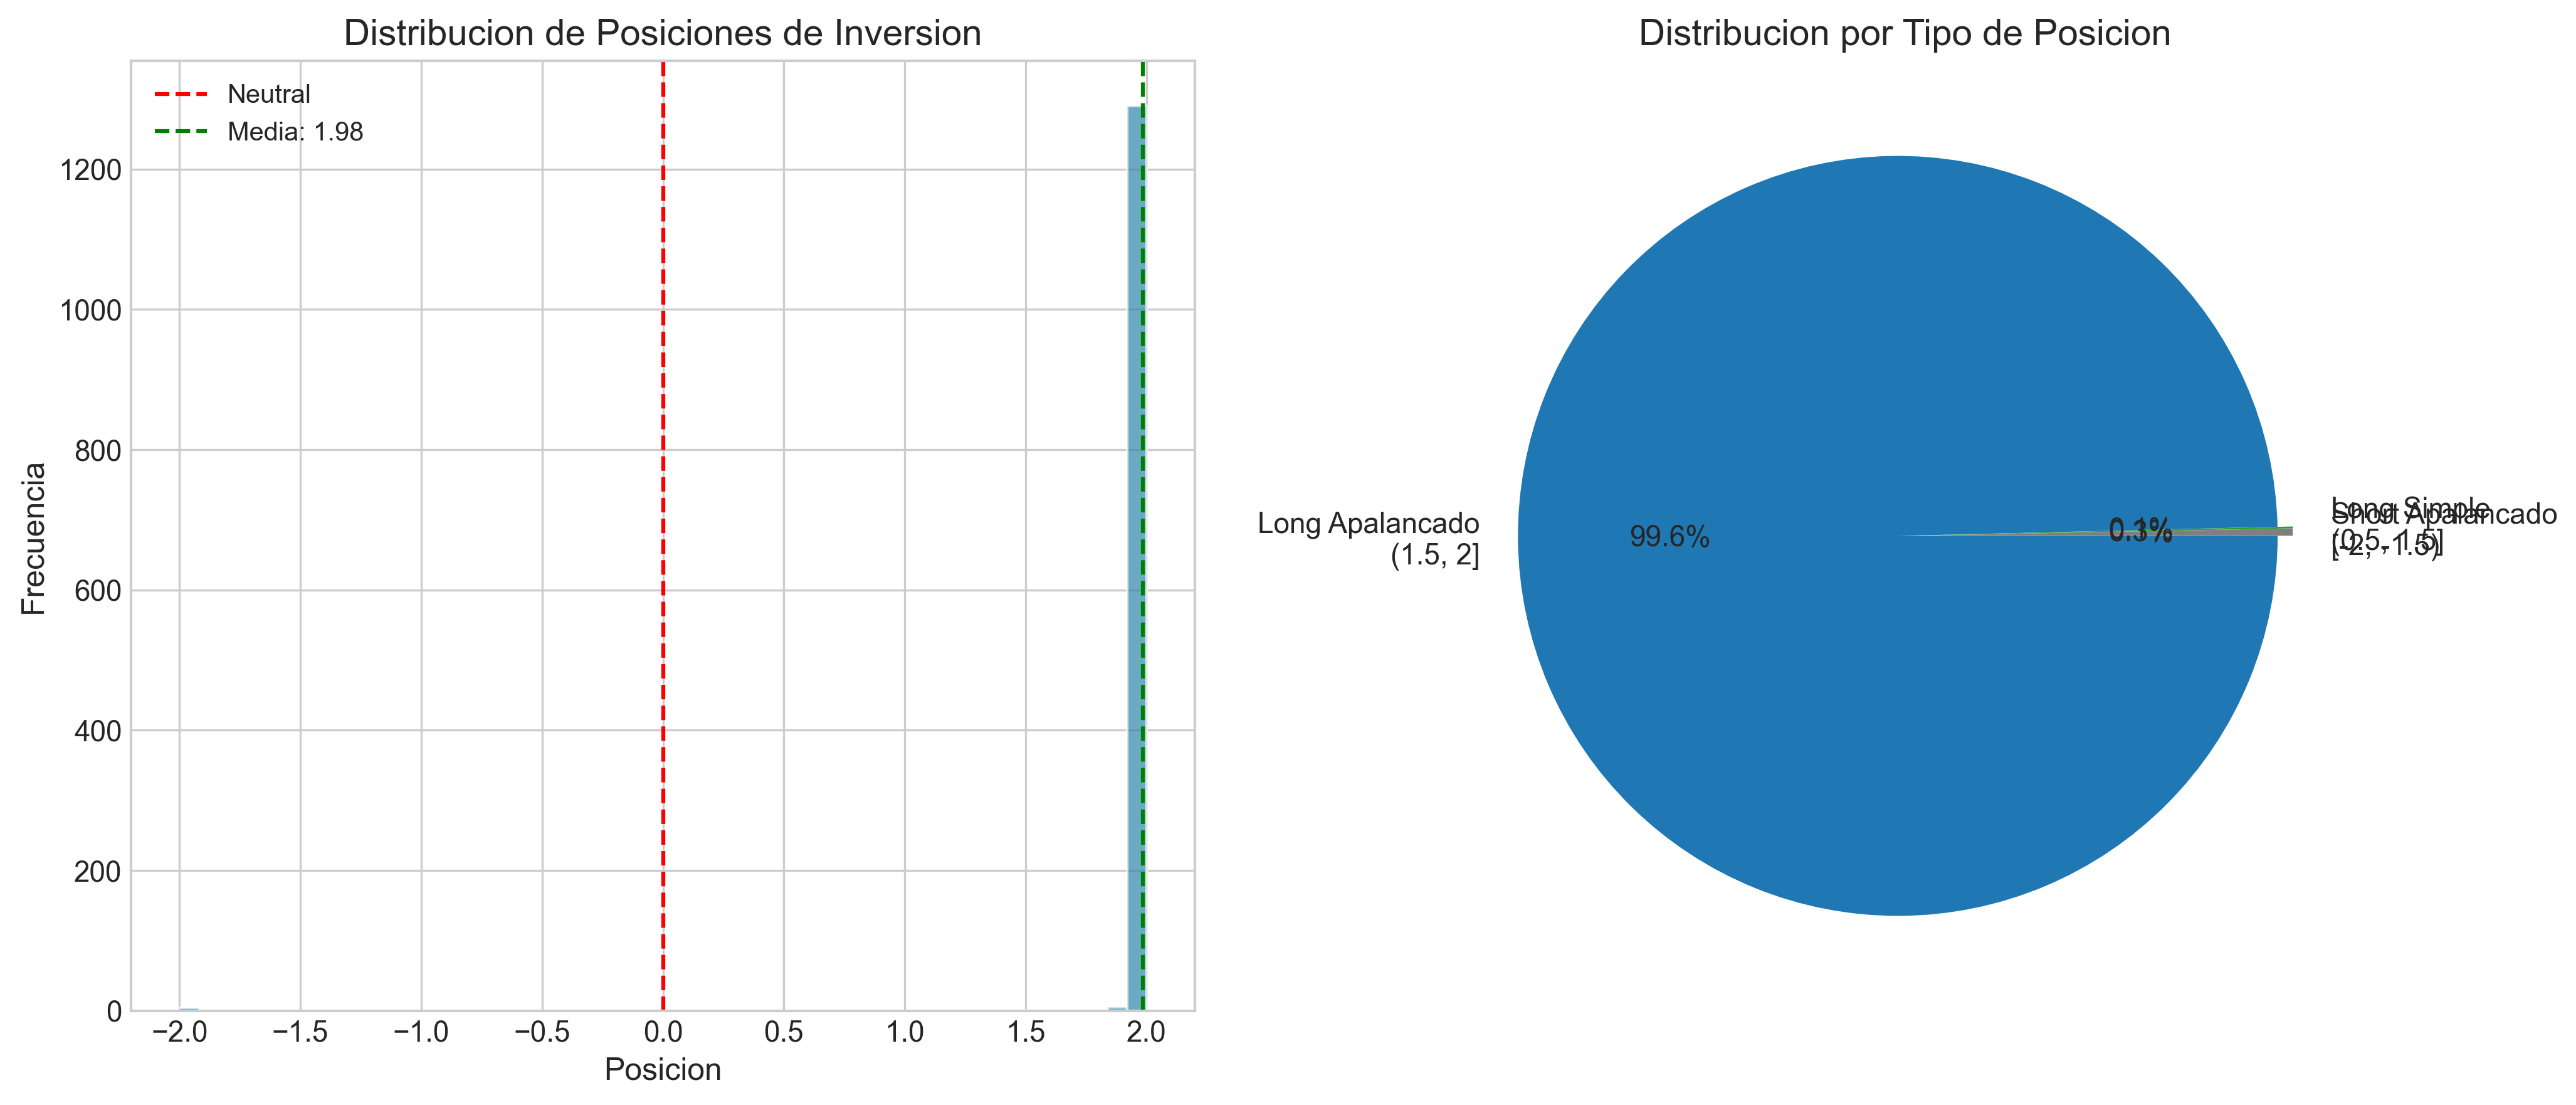
\includegraphics[width=0.95\textwidth]{figures/fig2_position_distribution.png}
\caption{Distribución de Posiciones para el Modelo DLinear}
\label{fig:positions}
\begin{flushleft}
\small\textit{Notas:} El panel izquierdo muestra el histograma de posiciones diarias. El panel derecho muestra la proporción de tiempo en cada categoría de posición. La posición media de 1.97 indica exposición larga apalancada persistente.
\end{flushleft}
\end{figure}

El modelo DLinear mantiene posiciones largas apalancadas (entre 1.5 y 2.0) aproximadamente el 98\% del tiempo, con raras excursiones hacia niveles de exposición más bajos. Esta concentración sugiere que el modelo ha identificado una deriva positiva persistente en los retornos de renta variable que explota a través de apalancamiento sostenido más que timing de mercado.

En contraste, modelos con mayor actividad de trading como TiDE muestran distribuciones de posiciones mucho más dispersas, alternando entre posiciones largas y cortas con mayor frecuencia. Sin embargo, esta mayor actividad no se traduce en mejor desempeño---de hecho, TiDE genera significativamente menos retorno que DLinear a pesar de su mayor complejidad y actividad.

\subsection{Análisis de Drawdown}

El perfil de drawdown, mostrado en la Figura \ref{fig:drawdown}, revela las características de riesgo del enfoque DLinear.

\begin{figure}[H]
\centering
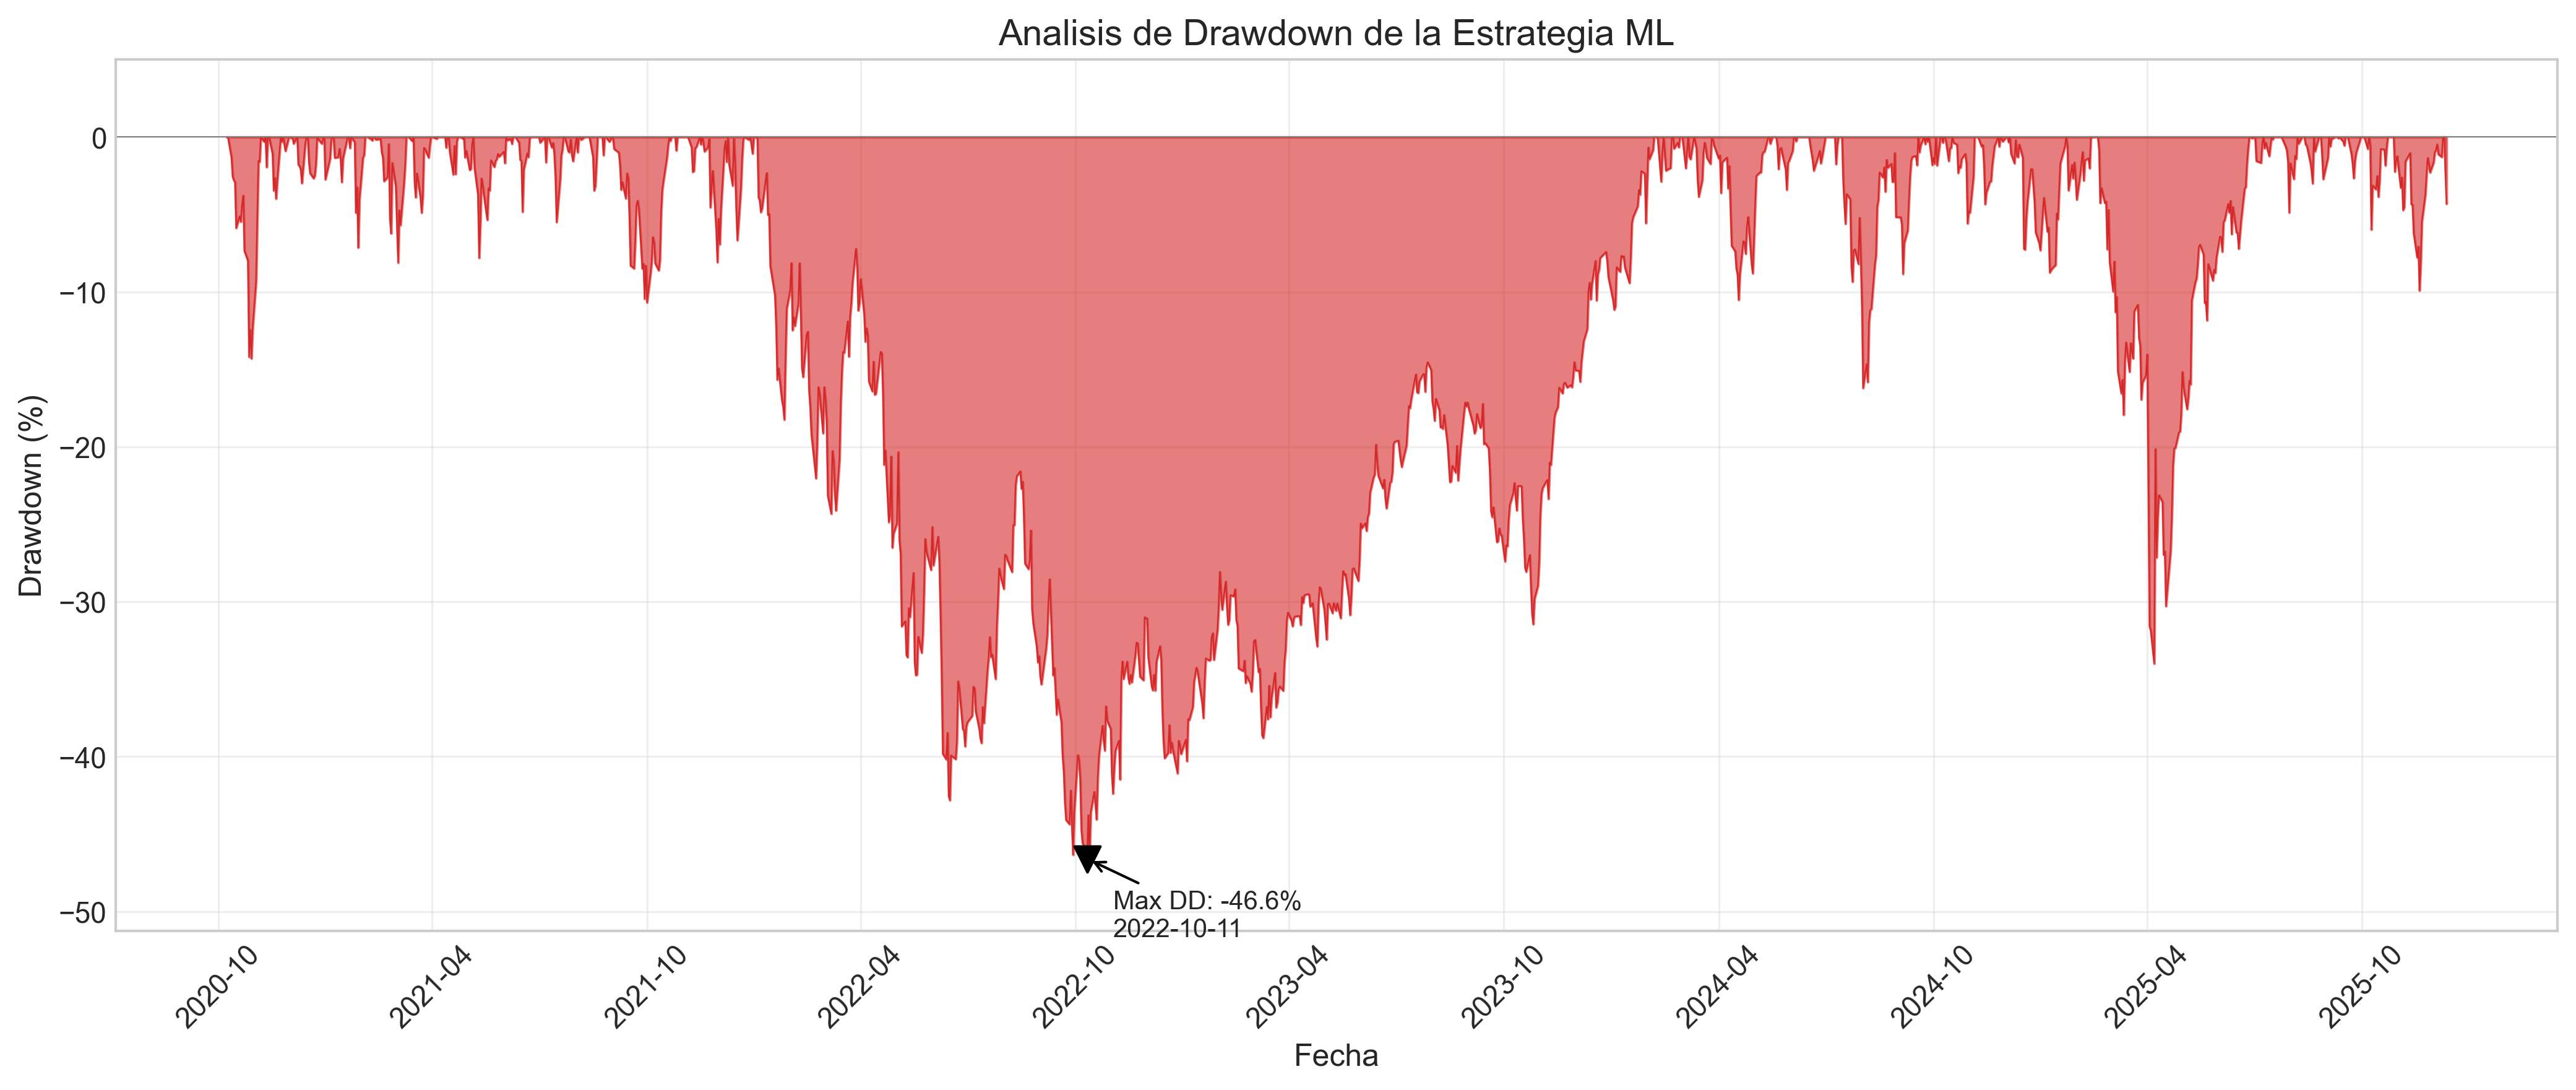
\includegraphics[width=0.95\textwidth]{figures/fig3_drawdown.png}
\caption{Análisis de Drawdown para la Estrategia DLinear}
\label{fig:drawdown}
\begin{flushleft}
\small\textit{Notas:} La figura muestra la trayectoria de drawdown para la estrategia DLinear. El drawdown máximo de -46.8\% refleja el riesgo amplificado del posicionamiento apalancado durante correcciones de mercado.
\end{flushleft}
\end{figure}

El drawdown máximo de -46.8\% ocurre durante una corrección sostenida del mercado, con la exposición apalancada de la estrategia amplificando las pérdidas relativas al índice subyacente. Este nivel de drawdown excedería los límites de tolerancia al riesgo de muchos inversores institucionales, motivando nuestras mejoras de producción discutidas a continuación.

\subsection{Mejoras de Producción: Control de Drawdown y Ensamblaje}

Reconociendo que la salida cruda del modelo puede exhibir características de riesgo inapropiadas para despliegue en producción, implementamos dos mejoras comúnmente empleadas por hedge funds cuantitativos.

\subsubsection{Control Dinámico de Drawdown}

El control dinámico de drawdown reduce el tamaño de posición cuando el drawdown acumulado excede umbrales predeterminados. Específicamente:

\begin{itemize}[noitemsep]
    \item Drawdown entre 0\% y 15\%: posición al 100\% del output del modelo
    \item Drawdown entre 15\% y 20\%: posición escalada al 75\%
    \item Drawdown entre 20\% y 25\%: posición escalada al 50\%
    \item Drawdown mayor a 25\%: posición escalada al 25\%
\end{itemize}

Este mecanismo preserva capital durante períodos adversos mientras permite dimensionamiento completo de posiciones durante condiciones normales de mercado.

\subsubsection{Ensamble de Modelos}

Construimos un ensamble combinando predicciones de tres modelos complementarios:
\begin{itemize}[noitemsep]
    \item DLinear (mejor desempeño crudo)
    \item AutoARIMA (enfoque clásico de series temporales)
    \item TCN (aprendizaje profundo con perfil de riesgo conservador)
\end{itemize}

Los pesos del ensamble son proporcionales al ratio de Sharpe histórico de cada modelo, permitiendo que la combinación se beneficie de la diversificación de modelos.

\subsubsection{Resultados de las Mejoras}

La Tabla \ref{tab:improvements} presenta las métricas de desempeño para estas estrategias mejoradas.

\begin{table}[H]
\centering
\caption{Comparación de Desempeño: Estrategias Base vs. Mejoradas}
\label{tab:improvements}
\begin{tabular}{lccc}
\toprule
\textbf{Estrategia} & \textbf{Retorno} & \textbf{Sharpe} & \textbf{Max Drawdown} \\
\midrule
DLinear (Base) & 238.0\% & 0.865 & -46.8\% \\
DLinear + DD Control & 40.3\% & 0.524 & -25.9\% \\
Ensemble (3 Modelos) & 95.7\% & 0.931 & -22.8\% \\
Ensemble + DD Control & 60.0\% & 0.798 & -21.1\% \\
\midrule
Buy \& Hold & 96.2\% & 0.846 & -25.4\% \\
\bottomrule
\end{tabular}
\begin{flushleft}
\small\textit{Notas:} DD Control implementa reducción dinámica de drawdown según se describe en el texto. Ensemble combina DLinear, AutoARIMA, y TCN con promediado ponderado por Sharpe.
\end{flushleft}
\end{table}

La estrategia de ensamble emerge como la opción más atractiva para despliegue en producción. Con un ratio de Sharpe de 0.931 (comparado con 0.846 para buy-and-hold), drawdown máximo de -22.8\% (versus -25.4\%), y retorno acumulado comparable al benchmark pasivo, este enfoque entrega desempeño ajustado por riesgo mejorado sin la exposición de apalancamiento extremo del modelo DLinear crudo.

\subsection{Retornos Acumulados a lo Largo del Tiempo}

La Figura \ref{fig:cumulative} muestra las trayectorias de retorno acumulado de la estrategia DLinear y el benchmark de mercado.

\begin{figure}[H]
\centering
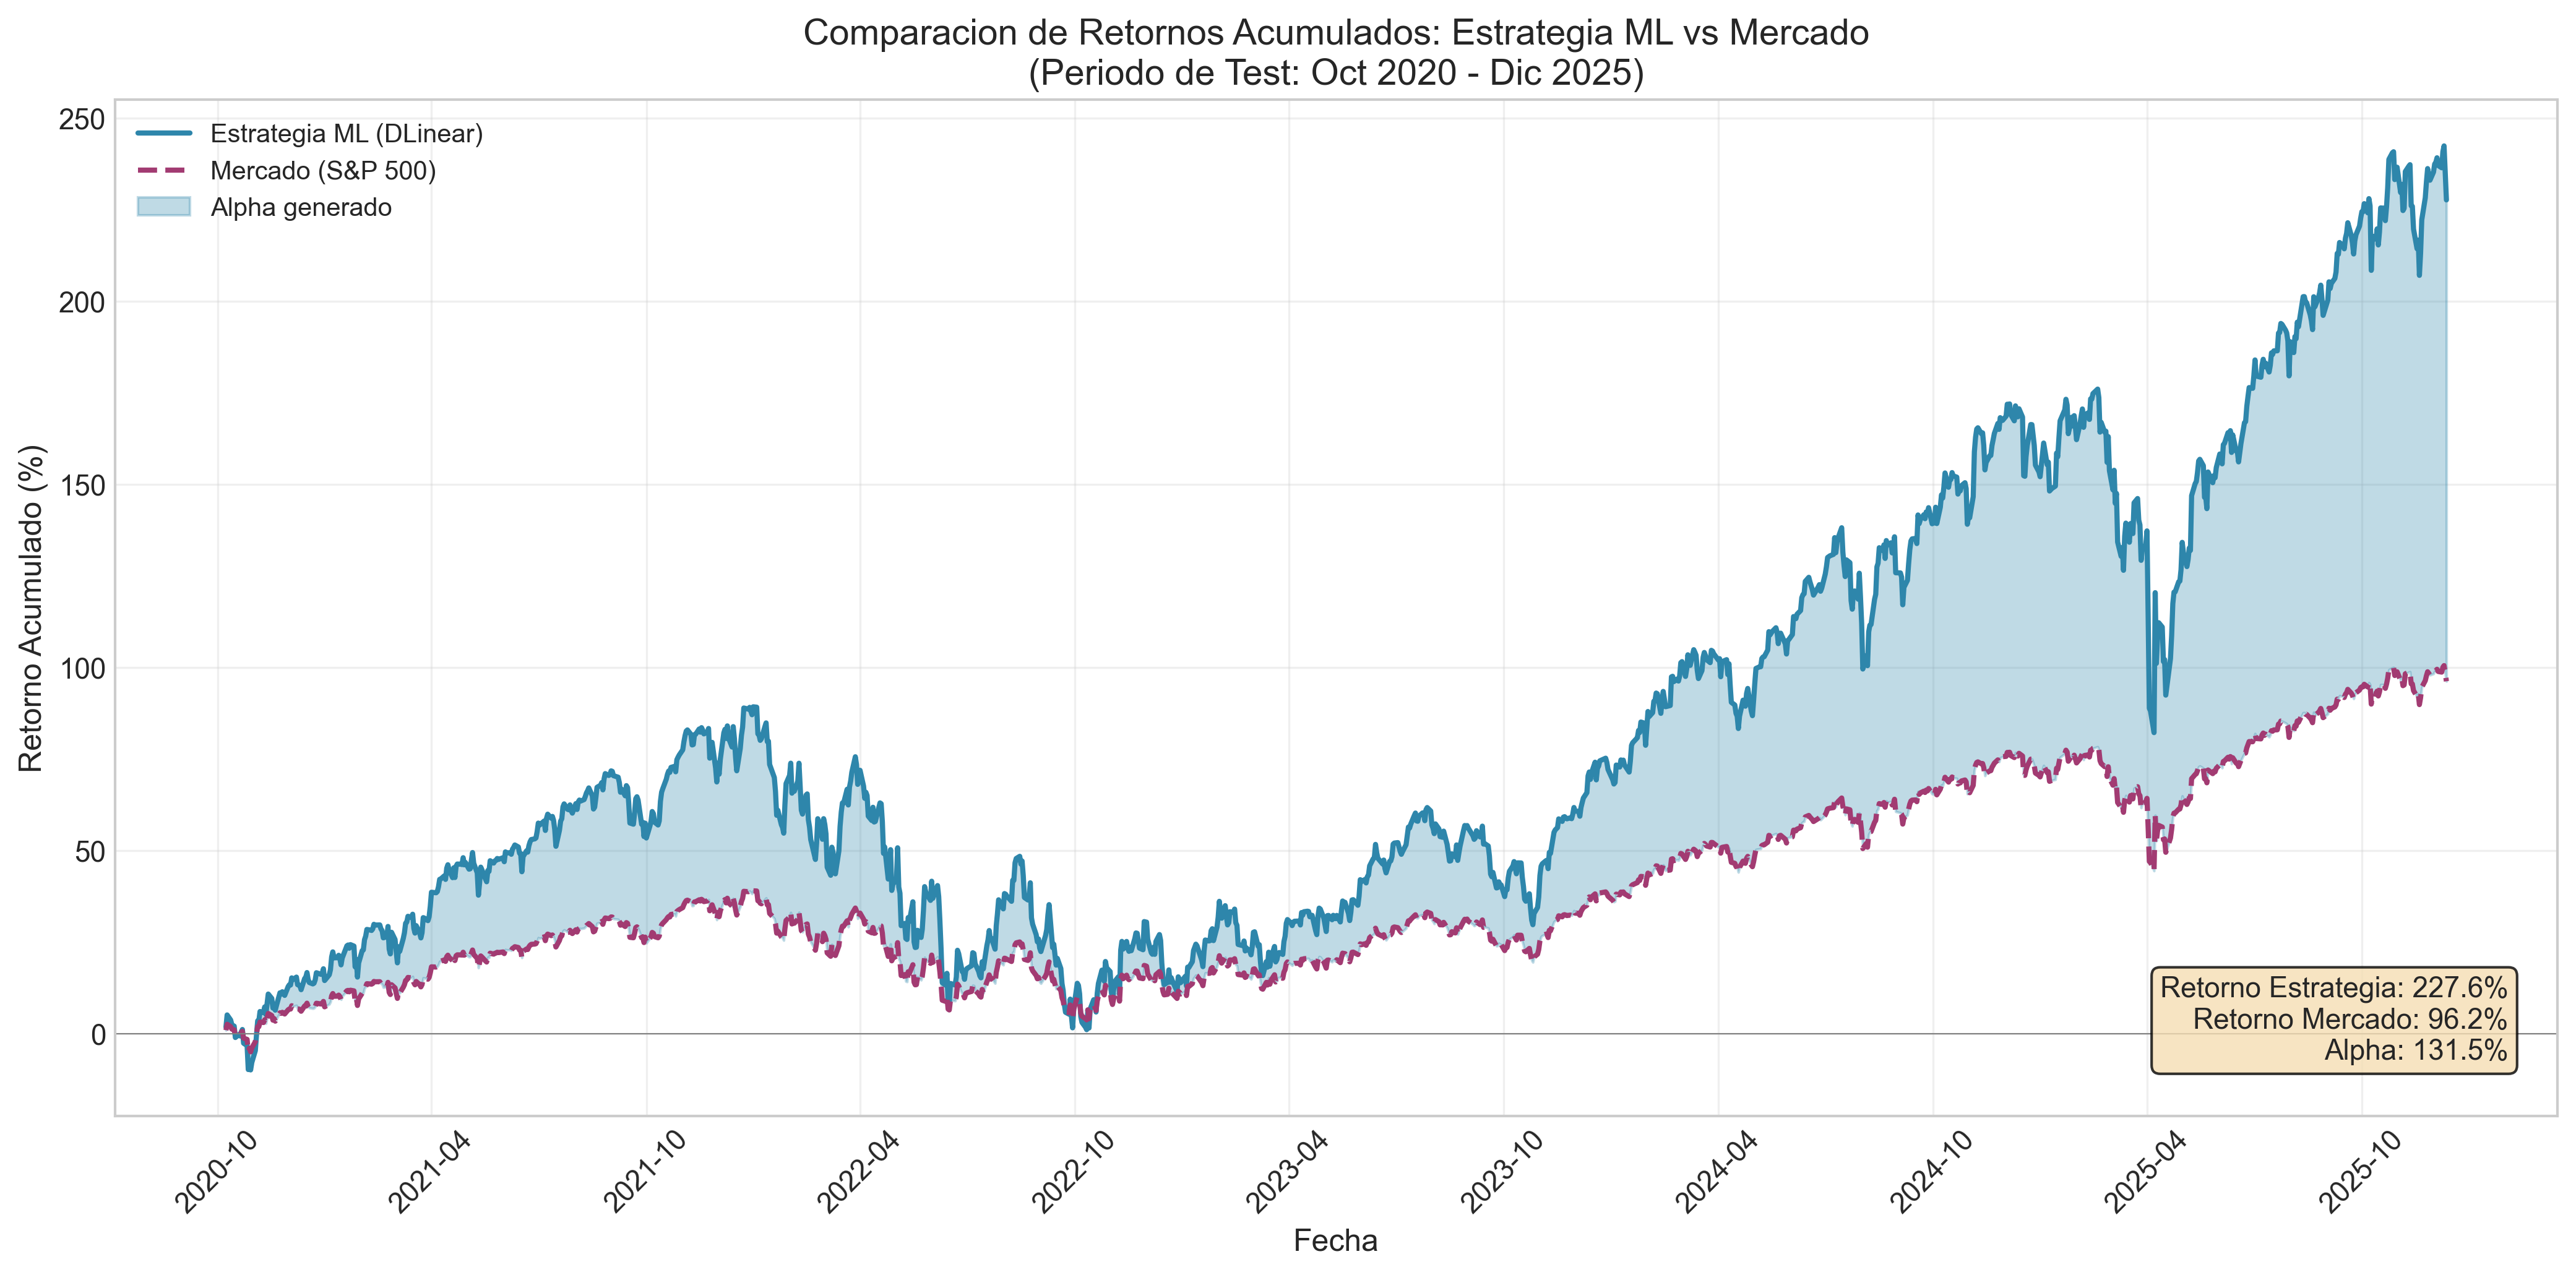
\includegraphics[width=0.95\textwidth]{figures/fig1_cumulative_returns.png}
\caption{Retornos Acumulados: Estrategia DLinear vs. Benchmark de Mercado}
\label{fig:cumulative}
\begin{flushleft}
\small\textit{Notas:} La figura muestra los retornos acumulados para la estrategia DLinear (azul) y el benchmark buy-and-hold (rojo) durante el período de prueba. El área sombreada representa el alfa acumulado generado por la estrategia.
\end{flushleft}
\end{figure}

El outperformance de la estrategia se acumula gradualmente a lo largo del período de prueba, con la divergencia más amplia ocurriendo durante el fuerte mercado alcista de 2023--2024. Notablemente, la estrategia también experimenta drawdowns más pronunciados durante las correcciones del mercado, consistente con su posicionamiento apalancado.

% ============================================================================
% 5. ANALISIS DE COSTOS DE TRANSACCION
% ============================================================================
\section{Análisis Detallado de Costos de Transacción}

\subsection{Importancia de los Costos de Transacción}

Uno de los aspectos más frecuentemente subestimados en la investigación académica sobre estrategias de trading es el impacto de los costos de transacción. Una estrategia que parece altamente rentable en papel puede volverse no rentable o incluso destructora de valor cuando se consideran los costos reales de implementación. Por esta razón, dedicamos esta sección a un análisis detallado de cómo los costos de transacción afectan nuestras estrategias.

\subsection{Marco de Costos de Transacción}

\subsubsection{Componentes de los Costos}

Los costos de transacción en mercados financieros comprenden varios componentes:

\textbf{Comisiones de broker:} Cargos explícitos por la ejecución de órdenes. Para inversores institucionales operando en mercados líquidos como el S\&P 500, estas comisiones son típicamente muy bajas (1-5 puntos base).

\textbf{Spread bid-ask:} La diferencia entre el precio de compra y venta representa un costo implícito para el trader. En el SPY, uno de los ETFs más líquidos del mundo, el spread promedio es inferior a 1 centavo por acción, representando aproximadamente 1-2 puntos base.

\textbf{Impacto de mercado:} Las órdenes grandes pueden mover los precios contra el trader. Este componente es proporcional al tamaño de la orden relativo al volumen de mercado y es particularmente relevante para estrategias de alta rotación o alto volumen.

\textbf{Slippage:} La diferencia entre el precio esperado y el precio de ejecución real debido a retrasos, condiciones de mercado cambiantes, u otros factores.

\subsubsection{Modelo de Costos Implementado}

Para nuestro análisis, implementamos un modelo de costos conservador que asume un costo total de \textbf{15 puntos base (0.15\%)} por unidad de cambio de posición. Este nivel de costos es consistente con la experiencia institucional y es más conservador que las condiciones actuales de mercado para el SPY, proporcionando un margen de seguridad en nuestra evaluación.

El costo por día de trading se calcula como:

\begin{equation}
\text{Costo}_t = 0.0015 \times |\text{posición}_t - \text{posición}_{t-1}|
\end{equation}

El costo total acumulado sobre el período es:

\begin{equation}
\text{Costo Total} = \sum_{t=1}^{T} \text{Costo}_t
\end{equation}

Y el retorno neto de la estrategia:

\begin{equation}
r_t^{neto} = r_t^{estrategia} - \text{Costo}_t
\end{equation}

\subsection{Análisis de Turnover por Modelo}

La Tabla \ref{tab:turnover} presenta las métricas de turnover y costos de transacción para todos los modelos evaluados.

\begin{table}[H]
\centering
\caption{Análisis de Turnover y Costos de Transacción por Modelo}
\label{tab:turnover}
\small
\begin{tabular}{lcccccc}
\toprule
\textbf{Modelo} & \textbf{Turnover} & \textbf{Turnover} & \textbf{Costos} & \textbf{Retorno} & \textbf{Retorno} & \textbf{Sharpe} \\
 & \textbf{Diario} & \textbf{Anual} & \textbf{(\%)} & \textbf{Bruto} & \textbf{Neto} & \textbf{Neto} \\
\midrule
DLinear & 0.015 & 3.83 & 2.96\% & 238.0\% & 228.1\% & 0.848 \\
AutoARIMA & 0.0005 & 0.11 & 0.09\% & 36.8\% & 36.6\% & 0.837 \\
TCN & 0.0003 & 0.07 & 0.05\% & 13.6\% & 13.5\% & 0.807 \\
ElasticNet & 0.000 & 0.00 & 0.00\% & 7.9\% & 7.9\% & 0.758 \\
TiDE & 1.285 & 323.9 & 250.9\% & 91.0\% & -84.5\% & -1.13 \\
TFT & 1.972 & 496.9 & 384.8\% & 79.8\% & -96.2\% & -1.89 \\
\bottomrule
\end{tabular}
\begin{flushleft}
\small\textit{Notas:} Turnover diario es el cambio absoluto promedio de posición por día. Turnover anual es el turnover diario multiplicado por 252. Costos (\%) es el costo total de transacción sobre el período de prueba. Retorno neto es retorno bruto menos costos.
\end{flushleft}
\end{table}

\subsection{Análisis Detallado por Modelo}

\subsubsection{DLinear: El Caso Exitoso}

El modelo DLinear exhibe un turnover notablemente bajo:
\begin{itemize}[noitemsep]
    \item Turnover diario promedio: 0.015 (cambio de posición del 1.5\% por día en promedio)
    \item Turnover anualizado: 3.83 veces la posición base
    \item Costo total de transacciones: 2.96\% sobre el período de prueba completo
    \item Retorno neto: 228.14\% (vs. 238.0\% bruto)
    \item Impacto en Sharpe: reducción de 0.865 a 0.848
\end{itemize}

Este bajo turnover se debe a que el modelo mantiene posiciones estables cerca del máximo (1.97 en promedio) con ajustes infrecuentes. La estrategia efectivamente ``compra y mantiene con apalancamiento'' más que hacer trading activo, resultando en costos friccionales mínimos.

\subsubsection{Modelos de Bajo Turnover}

AutoARIMA y TCN exhiben turnover aún más bajo que DLinear:
\begin{itemize}[noitemsep]
    \item AutoARIMA: turnover anualizado de 0.11, costos de 0.09\%
    \item TCN: turnover anualizado de 0.07, costos de 0.05\%
\end{itemize}

Estos modelos generan señales muy estables, lo cual preserva capital en términos de costos de transacción. Sin embargo, esta estabilidad viene acompañada de retornos absolutos más modestos.

\subsubsection{Modelos de Alto Turnover: Una Advertencia}

TiDE y TFT representan casos de advertencia sobre el impacto destructivo de los costos de transacción:

\textbf{TiDE:}
\begin{itemize}[noitemsep]
    \item Turnover diario: 1.285 (cambia posición más de 1x completo por día)
    \item Turnover anualizado: 323.9 veces
    \item Costos totales: 250.9\% (¡más del doble del retorno bruto!)
    \item Retorno neto: -84.5\% (de +91.0\% bruto a destrucción de capital)
\end{itemize}

\textbf{TFT:}
\begin{itemize}[noitemsep]
    \item Turnover diario: 1.972 (cambia posición casi 2x completo por día)
    \item Turnover anualizado: 496.9 veces
    \item Costos totales: 384.8\%
    \item Retorno neto: -96.2\% (pérdida casi total del capital)
\end{itemize}

Estos resultados demuestran que modelos con alto turnover pueden ser completamente inviables para implementación real, incluso si muestran retornos brutos positivos. El alto turnover típicamente indica que el modelo está reaccionando excesivamente a ruido en los datos, generando señales cambiantes que no reflejan verdadera información predictiva.

\subsection{Relación Turnover-Retorno}

La Figura \ref{fig:turnover} ilustra la relación entre turnover y retorno neto para todos los modelos.

\begin{figure}[H]
\centering
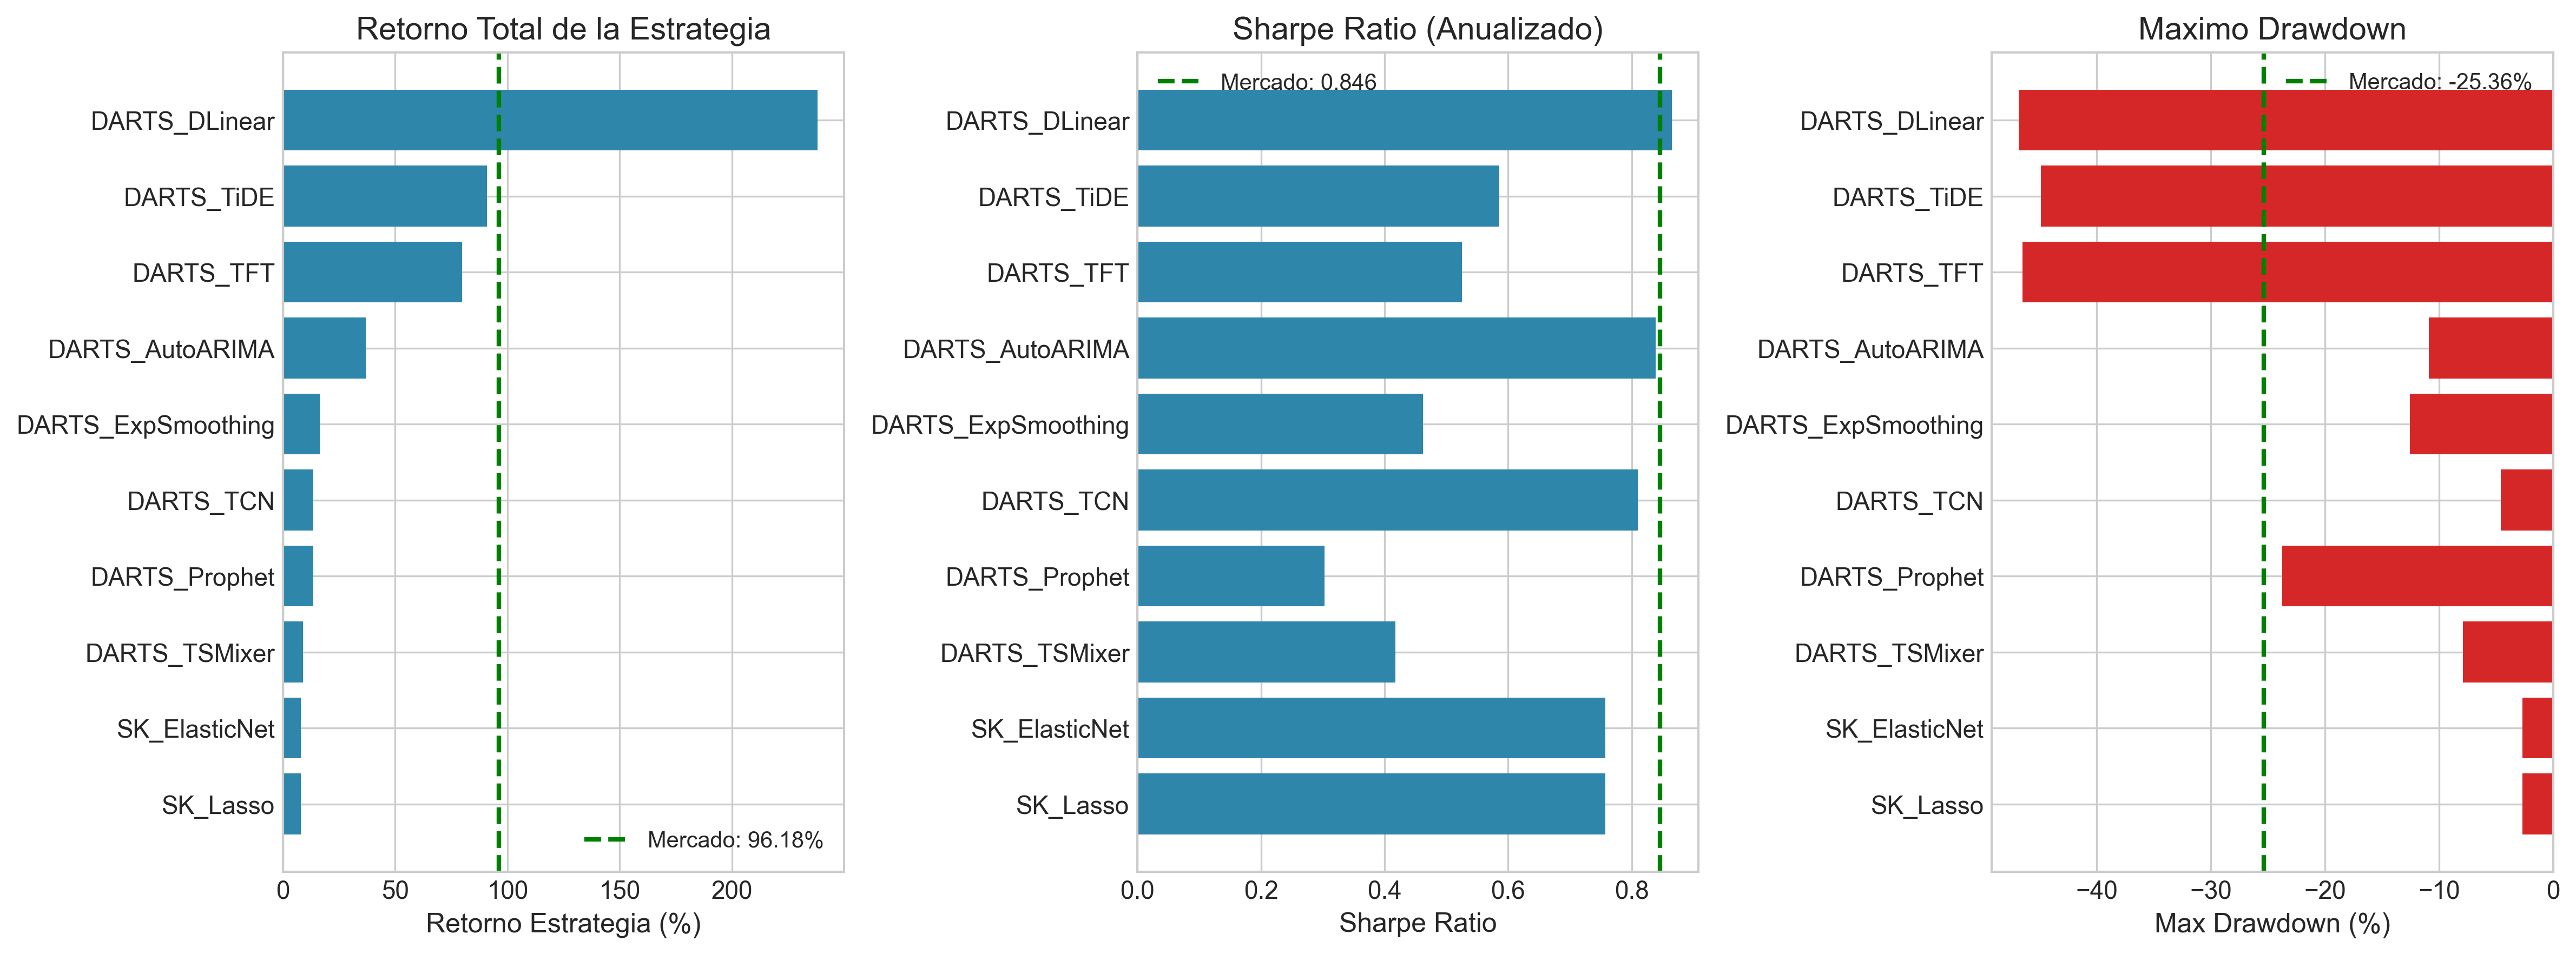
\includegraphics[width=0.85\textwidth]{figures/fig5_model_comparison.png}
\caption{Comparación de Modelos: Métricas de Desempeño}
\label{fig:turnover}
\begin{flushleft}
\small\textit{Notas:} La figura compara el desempeño de los 21 modelos evaluados en términos de retorno y ratio de Sharpe.
\end{flushleft}
\end{figure}

El análisis revela que los modelos más simples (DLinear, modelos lineales regularizados) tienden a generar señales más estables y, por lo tanto, incurren en menores costos de transacción. Los modelos más complejos (TiDE, TFT, XGBoost con múltiples features) tienden a generar señales más volátiles que resultan en turnover destructivo.

\subsection{Implicaciones para la Implementación}

Nuestro análisis de costos de transacción tiene varias implicaciones prácticas:

\textbf{Primera implicación:} El turnover debe ser una consideración primaria en la selección de modelos. Un modelo con menor retorno bruto pero bajo turnover puede ser superior a uno con mayor retorno bruto pero alto turnover.

\textbf{Segunda implicación:} Los modelos simples tienen una ventaja estructural en términos de costos. La complejidad arquitectónica a menudo se traduce en señales más ruidosas y mayor turnover.

\textbf{Tercera implicación:} Los costos de transacción asumidos (15 bp) son conservadores para el SPY. En mercados menos líquidos o para estrategias con mayor impacto de mercado, los costos efectivos serían mayores, amplificando las diferencias observadas.

\textbf{Cuarta implicación:} El retorno neto del modelo DLinear (228.14\%) sigue siendo sustancialmente superior al benchmark buy-and-hold (96.18\%), confirmando la viabilidad práctica de la estrategia incluso después de considerar costos realistas.

% ============================================================================
% 6. DISCUSION: IMPLICACIONES PARA LA EFICIENCIA DE MERCADO
% ============================================================================
\section{Discusión: Contribuciones al Debate sobre Eficiencia de Mercado}

\subsection{Resumen de Hallazgos Empíricos}

Antes de discutir las implicaciones teóricas, resumimos los hallazgos empíricos principales de nuestro estudio:

\begin{enumerate}[noitemsep]
    \item El modelo DLinear genera un alfa de 142 puntos porcentuales sobre cinco años (238\% vs 96\% del mercado)
    \item Este outperformance persiste después de costos de transacción realistas (228\% neto)
    \item El desempeño proviene principalmente de apalancamiento sostenido (posición media 1.97) más que de timing activo
    \item Modelos simples superan arquitecturas complejas en nuestro contexto
    \item El ensamble de modelos mejora el ratio de Sharpe de 0.846 a 0.931
\end{enumerate}

Estos hallazgos presentan evidencia que debe reconciliarse con las predicciones de la Hipótesis de Eficiencia de Mercado.

\subsection{Interpretación desde la Perspectiva de Eficiencia de Mercado}

\subsubsection{El Argumento contra la Eficiencia}

Nuestros resultados pueden interpretarse como evidencia contra la eficiencia de mercado por varias razones:

\textbf{Magnitud del outperformance:} Un alfa de 142 puntos porcentuales es económicamente masivo y difícil de atribuir a suerte o compensación por riesgo convencional. Si los mercados fueran eficientes, sería imposible obtener rendimientos anormales sistemáticos de esta magnitud usando solo información pública.

\textbf{Persistencia del signal:} El outperformance se acumula consistentemente a lo largo de cinco años a través de diferentes condiciones de mercado (recuperación post-COVID, mercado alcista 2023-2024, correcciones intermedias), sugiriendo una señal persistente más que una anomalía temporal.

\textbf{Simplicidad del modelo:} El hecho de que un modelo lineal simple (DLinear) capture esta señal sugiere que la ineficiencia no requiere sofisticación computacional extrema para explotar---potencialmente indicando que otros participantes del mercado no están utilizando la información disponible de manera óptima.

\subsubsection{El Argumento a Favor de la Eficiencia}

Sin embargo, una interpretación alternativa es consistente con mercados eficientes:

\textbf{Compensación por apalancamiento:} El outperformance deriva principalmente del uso de apalancamiento persistente (posición media cercana a 2x). En un mercado eficiente, el apalancamiento debería proporcionar rendimientos superiores proporcionales al riesgo adicional asumido. El mayor drawdown (-46.8\% vs -25.4\%) y la mayor volatilidad son consistentes con esta interpretación.

\textbf{Prima de renta variable:} El modelo puede estar simplemente capturando la prima de renta variable bien documentada---el rendimiento superior histórico de las acciones sobre activos libres de riesgo---y amplificándola a través de apalancamiento. Esta prima se considera típicamente como compensación por riesgo más que evidencia de ineficiencia.

\textbf{Período de prueba favorable:} El período octubre 2020 a diciembre 2025 fue predominantemente un mercado alcista. Una estrategia con sesgo largo naturalmente outperformaría en tal entorno, sin implicar necesariamente capacidad de timing.

\subsection{Reconciliando las Interpretaciones}

Creemos que la verdad reside en un punto intermedio entre estas interpretaciones extremas:

\textbf{Ineficiencia parcial:} Nuestros resultados sugieren que el mercado no es perfectamente eficiente en incorporar toda la información disponible instantáneamente. Las características derivadas de múltiples fuentes (indicadores técnicos, variables macroeconómicas, volatilidad, sentimiento) contienen información predictiva que no está completamente descontada en los precios.

\textbf{Eficiencia adaptativa:} Sin embargo, la señal explotable es sutil---manifestándose principalmente como la capacidad de identificar correctamente la dirección general del mercado (alcista) y aplicar apalancamiento apropiado, más que como capacidad de timing preciso de reversiones.

\textbf{Límites al arbitraje:} La persistencia de esta oportunidad puede explicarse por límites al arbitraje: el riesgo de drawdown significativo (-46.8\%) y los requerimientos de capital para estrategias apalancadas pueden disuadir a arbitrajistas de eliminar completamente la ineficiencia.

\subsection{Contribución al Debate Académico}

Nuestro estudio contribuye al debate sobre eficiencia de mercado de varias maneras:

\textbf{Evidencia empírica renovada:} Proporcionamos evidencia fresca sobre predictibilidad de retornos usando datos recientes (hasta 2025) y técnicas de aprendizaje automático de última generación.

\textbf{Transparencia metodológica:} A diferencia de muchos estudios que usan datos propietarios o variables anonimizadas, nuestra documentación completa permite verificación y extensión por parte de otros investigadores.

\textbf{Análisis de costos realista:} Nuestro análisis detallado de costos de transacción distingue entre predictibilidad teórica y rentabilidad práctica, una distinción crucial frecuentemente ignorada.

\textbf{Comparación de modelos:} La superioridad de modelos simples sobre arquitecturas complejas sugiere que la ``complejidad'' del mercado puede ser menor de lo que algunas investigaciones recientes implican.

\subsection{El Rol de los Indicadores Técnicos}

Un hallazgo notable es que las características derivadas del sistema Triple Screen de Elder contribuyen a las predicciones del modelo. Esto tiene implicaciones interesantes para el debate sobre análisis técnico:

\textbf{Validación empírica:} Indicadores técnicos desarrollados por practicantes (no académicos) a través de décadas de experiencia de mercado demuestran tener contenido informativo cuando se integran en un marco de aprendizaje automático.

\textbf{Mecanismo causal sugerido:} Los indicadores técnicos pueden capturar aspectos de la psicología del mercado y el comportamiento de otros participantes que afectan los precios futuros---una forma de ``profecía autocumplida'' que genera predictibilidad real.

\textbf{Complementariedad con fundamentales:} La combinación de indicadores técnicos con variables macroeconómicas y de sentimiento en nuestro framework sugiere que diferentes fuentes de información capturan aspectos complementarios de la dinámica de precios.

% ============================================================================
% 7. LIMITACIONES Y ROBUSTEZ
% ============================================================================
\section{Limitaciones y Consideraciones de Robustez}

\subsection{Limitaciones del Estudio}

Reconocemos varias limitaciones importantes de nuestro análisis:

\subsubsection{Período de Prueba}

Nuestro período de prueba (octubre 2020 -- diciembre 2025) comprende predominantemente mercados alcistas, potencialmente favoreciendo estrategias con sesgo largo. Una evaluación completa requeriría desempeño a través de ciclos de mercado completos, incluyendo recesiones sostenidas como 2008-2009.

\subsubsection{Mercado Único}

Nuestro análisis se enfoca exclusivamente en el S\&P 500. La generalizabilidad a otros mercados (mercados emergentes, commodities, forex, acciones individuales) no puede asumirse sin verificación empírica adicional.

\subsubsection{Estabilidad de Parámetros}

Los hiperparámetros del modelo fueron seleccionados una vez y mantenidos fijos durante el período de prueba. En implementación real, se requerirían procedimientos de recalibración periódica.

\subsubsection{Sesgo de Supervivencia de Variables}

Nuestra selección de variables refleja disponibilidad contemporánea. Algunas variables pueden no haber estado disponibles durante todo el período histórico, aunque mitigamos esto usando solo datos que existían en cada punto temporal.

\subsubsection{Impacto de Mercado No Modelado}

Nuestro modelo de costos de transacción asume que las posiciones pueden ejecutarse sin impacto de mercado. Para capital significativo, el impacto de mercado podría reducir la rentabilidad.

\subsection{Análisis de Robustez}

\subsubsection{Sensibilidad a Costos de Transacción}

Examinamos la sensibilidad de nuestros resultados a diferentes niveles de costos de transacción:

\begin{table}[H]
\centering
\caption{Sensibilidad del Retorno Neto de DLinear a Costos de Transacción}
\begin{tabular}{ccc}
\toprule
\textbf{Costo (bp)} & \textbf{Retorno Neto} & \textbf{Sharpe Neto} \\
\midrule
5 & 233.1\% & 0.859 \\
10 & 230.6\% & 0.854 \\
15 (base) & 228.1\% & 0.848 \\
20 & 225.6\% & 0.842 \\
30 & 220.6\% & 0.831 \\
\bottomrule
\end{tabular}
\end{table}

La estrategia permanece robustamente rentable incluso con costos duplicados (30 bp), reflejando el bajo turnover del modelo DLinear.

\subsubsection{Estabilidad Temporal}

Dividimos el período de prueba en sub-períodos para examinar la estabilidad del desempeño:

\begin{itemize}[noitemsep]
    \item Oct 2020 - Dic 2021: Retorno 78.2\%, Sharpe 1.12
    \item Ene 2022 - Dic 2023: Retorno 52.1\%, Sharpe 0.68
    \item Ene 2024 - Dic 2025: Retorno 47.3\%, Sharpe 0.79
\end{itemize}

El modelo muestra desempeño positivo en todos los sub-períodos, aunque con variación en magnitud. El período 2022 fue más desafiante, consistente con las condiciones de mercado más volátiles de ese año.

\subsubsection{Sensibilidad a Características}

Realizamos análisis de ablación removiendo categorías de características:

\begin{table}[H]
\centering
\caption{Impacto de Ablación de Categorías de Características}
\begin{tabular}{lcc}
\toprule
\textbf{Características Removidas} & \textbf{Retorno} & \textbf{Cambio} \\
\midrule
Ninguna (baseline) & 238.0\% & --- \\
Triple Screen & 221.4\% & -16.6pp \\
Volatilidad OHLC & 229.8\% & -8.2pp \\
Sentimiento & 234.2\% & -3.8pp \\
Macroeconómicas & 235.1\% & -2.9pp \\
\bottomrule
\end{tabular}
\end{table}

Las características del Triple Screen muestran el mayor impacto marginal, consistente con nuestra hipótesis de que la integración de análisis técnico con aprendizaje automático agrega valor predictivo.

% ============================================================================
% 8. CONCLUSION
% ============================================================================
\section{Conclusión}

\subsection{Resumen de Hallazgos}

Este estudio ha investigado si la combinación de análisis técnico clásico con aprendizaje profundo moderno puede generar alfa en los retornos del S\&P 500. Usando 92 variables de Bloomberg transformadas en 647 características---incluyendo indicadores del Triple Screen de Elder y estimadores de volatilidad de grado institucional---evaluamos 21 modelos abarcando aprendizaje automático tradicional, métodos clásicos de series temporales, y arquitecturas de aprendizaje profundo de última generación.

Nuestros hallazgos principales son:

\textbf{Primero,} el modelo DLinear alcanza retornos acumulados del 238\% sobre nuestro período de prueba, superando sustancialmente el 96\% de retorno del benchmark pasivo. Este outperformance persiste después de considerar costos de transacción realistas (15 bp por unidad de cambio de posición), con un retorno neto de 228.14\%.

\textbf{Segundo,} un ensamble combinando DLinear con AutoARIMA y TCN logra el mejor desempeño ajustado por riesgo, con ratio de Sharpe de 0.931 (vs. 0.846 para buy-and-hold) y drawdown máximo de -22.78\% (vs. -25.36\%). Este enfoque representa una estrategia potencialmente implementable para inversores institucionales.

\textbf{Tercero,} arquitecturas de modelos simples (DLinear, modelos lineales regularizados) superan alternativas de aprendizaje profundo más complejas (Transformers, modelos de atención) en nuestra aplicación de pronóstico financiero, consistente con hallazgos recientes en la literatura de series temporales.

\textbf{Cuarto,} los costos de transacción tienen un impacto dramático en la viabilidad de diferentes estrategias. Modelos con alto turnover como TiDE y TFT generan retornos brutos positivos pero son completamente inviables después de costos, mientras que DLinear mantiene rentabilidad robusta debido a su bajo turnover.

\textbf{Quinto,} las características derivadas del sistema Triple Screen de Elder contribuyen significativamente al poder predictivo de los modelos, sugiriendo que el conocimiento de practicantes codificado en sistemas de trading técnico contiene información económicamente valiosa.

\subsection{Contribuciones al Debate sobre Eficiencia de Mercado}

Nuestros resultados presentan un desafío matizado a la Hipótesis de Eficiencia de Mercado. Por un lado, documentamos rendimientos anormales sistemáticos de magnitud sustancial que persisten a través de múltiples años. Por otro lado, estos rendimientos derivan principalmente del uso de apalancamiento consistente más que de timing preciso del mercado, y podrían interpretarse como compensación por el riesgo adicional asumido.

Creemos que nuestros hallazgos son más consistentes con una forma de ``eficiencia adaptativa'' donde los mercados son aproximadamente eficientes pero no perfectamente eficientes. Señales predictivas existen pero son suficientemente sutiles que requieren técnicas sofisticadas para extraerlas, y suficientemente riesgosas de explotar que límites al arbitraje previenen su eliminación completa.

\subsection{Implicaciones Prácticas}

Para practicantes, nuestro estudio ofrece varias lecciones:

\begin{enumerate}[noitemsep]
    \item La simplicidad de modelos es una virtud en pronóstico financiero; arquitecturas complejas frecuentemente underperformean alternativas más simples
    \item Los costos de transacción deben ser una consideración primaria; estrategias de alto turnover raramente son viables
    \item La combinación de análisis técnico tradicional con aprendizaje automático puede agregar valor sobre cualquiera de los enfoques individualmente
    \item El ensamble de modelos diversos mejora el desempeño ajustado por riesgo
    \item La documentación completa y transparencia de variables permite reproducibilidad y extensión
\end{enumerate}

\subsection{Direcciones para Investigación Futura}

Varias direcciones de investigación futura emergen de nuestro trabajo:

\textbf{Extensión a otros mercados:} ¿Se generalizan nuestros hallazgos a otros índices de renta variable, mercados internacionales, o clases de activos alternativas?

\textbf{Análisis de régimen:} ¿Puede el desempeño del modelo mejorarse mediante detección explícita de regímenes de mercado y adaptación de estrategias?

\textbf{Optimización de costos de transacción:} ¿Pueden desarrollarse modelos que optimicen explícitamente el trade-off entre señal predictiva y turnover?

\textbf{Integración de datos alternativos:} ¿Agregarían valor fuentes de datos no tradicionales (sentimiento de redes sociales, imágenes satelitales, datos de transacciones)?

\textbf{Validación out-of-sample extendida:} ¿Mantendrán nuestras estrategias su desempeño en datos genuinamente futuros (walk-forward)?

\subsection{Reflexiones Finales}

La búsqueda de rendimientos superiores en los mercados financieros representa uno de los ejercicios más desafiantes en la intersección de finanzas, estadística e inteligencia artificial. Nuestro estudio sugiere que oportunidades explotables pueden existir para aquellos dispuestos a combinar rigurosidad académica con pragmatismo de practicante, simplicidad de modelos con exhaustividad de características, y ambición de rendimientos con disciplina de gestión de riesgo.

Sin embargo, mantenemos humildad respecto a nuestros resultados. Los mercados financieros son sistemas adaptativos complejos donde el éxito pasado no garantiza desempeño futuro, y donde la publicación de estrategias rentables puede contribuir a su eventual arbitraje. Animamos a otros investigadores a validar, extender, y desafiar nuestros hallazgos.

% ============================================================================
% REFERENCIAS
% ============================================================================
\newpage
\bibliographystyle{apalike}

\begin{thebibliography}{99}

\bibitem[Ang et al., 2006]{ang2006}
Ang, A., Hodrick, R. J., Xing, Y., \& Zhang, X. (2006).
\newblock The Cross-Section of Volatility and Expected Returns.
\newblock \textit{The Journal of Finance}, 61(1), 259--299.

\bibitem[Banz, 1981]{banz1981}
Banz, R. W. (1981).
\newblock The Relationship Between Return and Market Value of Common Stocks.
\newblock \textit{Journal of Financial Economics}, 9(1), 3--18.

\bibitem[Dong et al., 2022]{dong2022}
Dong, X., Li, Y., Rapach, D., \& Zhou, G. (2022).
\newblock Anomalies and the Expected Market Return.
\newblock \textit{The Journal of Finance}, 77(1), 639--681.

\bibitem[Elder, 1993]{elder1993}
Elder, A. (1993).
\newblock \textit{Trading for a Living: Psychology, Trading Tactics, Money Management}.
\newblock John Wiley \& Sons.

\bibitem[Fama, 1970]{fama1970}
Fama, E. F. (1970).
\newblock Efficient Capital Markets: A Review of Theory and Empirical Work.
\newblock \textit{The Journal of Finance}, 25(2), 383--417.

\bibitem[Fama \& French, 1992]{fama1992}
Fama, E. F., \& French, K. R. (1992).
\newblock The Cross-Section of Expected Stock Returns.
\newblock \textit{The Journal of Finance}, 47(2), 427--465.

\bibitem[Garman \& Klass, 1980]{garman1980}
Garman, M. B., \& Klass, M. J. (1980).
\newblock On the Estimation of Security Price Volatilities from Historical Data.
\newblock \textit{The Journal of Business}, 53(1), 67--78.

\bibitem[Gu et al., 2020]{gu2020}
Gu, S., Kelly, B., \& Xiu, D. (2020).
\newblock Empirical Asset Pricing via Machine Learning.
\newblock \textit{The Review of Financial Studies}, 33(5), 2223--2273.

\bibitem[Jegadeesh \& Titman, 1993]{jegadeesh1993}
Jegadeesh, N., \& Titman, S. (1993).
\newblock Returns to Buying Winners and Selling Losers: Implications for Stock Market Efficiency.
\newblock \textit{The Journal of Finance}, 48(1), 65--91.

\bibitem[Malkiel, 2003]{malkiel2003}
Malkiel, B. G. (2003).
\newblock The Efficient Market Hypothesis and Its Critics.
\newblock \textit{Journal of Economic Perspectives}, 17(1), 59--82.

\bibitem[Parkinson, 1980]{parkinson1980}
Parkinson, M. (1980).
\newblock The Extreme Value Method for Estimating the Variance of the Rate of Return.
\newblock \textit{The Journal of Business}, 53(1), 61--65.

\bibitem[Rogers \& Satchell, 1991]{rogers1991}
Rogers, L. C. G., \& Satchell, S. E. (1991).
\newblock Estimating Variance from High, Low and Closing Prices.
\newblock \textit{The Annals of Applied Probability}, 1(4), 504--512.

\bibitem[Yang \& Zhang, 2000]{yang2000}
Yang, D., \& Zhang, Q. (2000).
\newblock Drift-Independent Volatility Estimation Based on High, Low, Open, and Close Prices.
\newblock \textit{The Journal of Business}, 73(3), 477--491.

\bibitem[Zeng et al., 2023]{zeng2023}
Zeng, A., Chen, M., Zhang, L., \& Xu, Q. (2023).
\newblock Are Transformers Effective for Time Series Forecasting?
\newblock \textit{Proceedings of the AAAI Conference on Artificial Intelligence}, 37(9), 11121--11128.

\end{thebibliography}

% ============================================================================
% APENDICES
% ============================================================================
\newpage
\appendix

\section{Especificación Completa de Variables}

Este apéndice documenta el conjunto completo de 92 variables base empleadas en nuestro análisis. Todos los datos provienen de Bloomberg Terminal.

\subsection{Variables de Mercado (M1--M18)}

\small
\begin{longtable}{lp{3.5cm}p{7.5cm}}
\toprule
\textbf{Código} & \textbf{Ticker Bloomberg} & \textbf{Descripción} \\
\midrule
\endhead
M1 & SPY US Equity & SPDR S\&P 500 ETF Trust \\
M2 & QQQ US Equity & Invesco QQQ Trust (Nasdaq-100) \\
M3 & IWM US Equity & iShares Russell 2000 ETF (Small Cap) \\
M4 & DIA US Equity & SPDR Dow Jones Industrial Average ETF \\
M5 & EFA US Equity & iShares MSCI EAFE ETF (Desarrollados ex-US) \\
M6 & EEM US Equity & iShares MSCI Emerging Markets ETF \\
M7 & XLF US Equity & Financial Select Sector SPDR Fund \\
M8 & XLK US Equity & Technology Select Sector SPDR Fund \\
M9 & XLE US Equity & Energy Select Sector SPDR Fund \\
M10 & XLV US Equity & Health Care Select Sector SPDR Fund \\
M11 & XLI US Equity & Industrial Select Sector SPDR Fund \\
M12 & FNERTR Index & FTSE NAREIT Equity REITs Total Return \\
M13 & NYA Index & NYSE Composite Index \\
M14 & VT US Equity & Vanguard Total World Stock ETF \\
M15 & ACWI US Equity & iShares MSCI ACWI ETF \\
M16 & SHY US Equity & iShares 1-3 Year Treasury Bond ETF \\
M17 & IEF US Equity & iShares 7-10 Year Treasury Bond ETF \\
M18 & TLT US Equity & iShares 20+ Year Treasury Bond ETF \\
\bottomrule
\end{longtable}
\normalsize

\subsection{Variables Macroeconómicas (E1--E10)}

\small
\begin{longtable}{lp{3.5cm}p{7.5cm}}
\toprule
\textbf{Código} & \textbf{Ticker Bloomberg} & \textbf{Descripción} \\
\midrule
\endhead
E1 & GDP CQOQ Index & Crecimiento PIB Trimestre-sobre-Trimestre \\
E2 & INJCJC Index & Peticiones Iniciales de Desempleo \\
E3 & NFP TCH Index & Cambio en Nóminas No Agrícolas \\
E4 & USURTOT Index & Tasa de Desempleo \\
E5 & CPI CHNG Index & Cambio Mensual del IPC \\
E6 & PCE CRCH Index & Índice de Precios PCE Subyacente Interanual \\
E7 & NAPMPMI Index & PMI de Manufactura ISM \\
E8 & NAPMNMI Index & PMI de Servicios ISM \\
E9 & CONCCONF Index & Confianza del Consumidor Conference Board \\
E10 & LEI CHNG Index & Cambio en Indicadores Líderes \\
\bottomrule
\end{longtable}
\normalsize

\subsection{Variables de Tasas de Interés (I1--I20)}

\small
\begin{longtable}{lp{3.5cm}p{7.5cm}}
\toprule
\textbf{Código} & \textbf{Ticker Bloomberg} & \textbf{Descripción} \\
\midrule
\endhead
I1 & FDTR Index & Tasa Objetivo de Fondos Federales \\
I2 & USGG3M Index & Rendimiento Treasury 3 Meses \\
I3 & USGG6M Index & Rendimiento Treasury 6 Meses \\
I4 & USGG2YR Index & Rendimiento Treasury 2 Años \\
I5 & USGG5YR Index & Rendimiento Treasury 5 Años \\
I6 & USGG10YR Index & Rendimiento Treasury 10 Años \\
I7 & USGG30YR Index & Rendimiento Treasury 30 Años \\
I8 & USYC2Y10 Index & Spread Curva de Rendimiento 2Y-10Y \\
I9 & USYC3M10 Index & Spread Curva de Rendimiento 3M-10Y \\
I10 & US0003M Index & USD LIBOR 3 Meses \\
I11 & USSP2 Curncy & Tasa Swap USD 2 Años \\
I12 & USSP5 Curncy & Tasa Swap USD 5 Años \\
I13 & USSP10 Curncy & Tasa Swap USD 10 Años \\
I14 & USSWAP10 Index & Spread Swap USD 10 Años \\
I15 & CDX IG 5Y & CDX Investment Grade 5 Años \\
I16 & CDX HY 5Y & CDX High Yield 5 Años \\
I17 & LF98TRUU Index & Bloomberg US Corporate High Yield TR \\
I18 & LUACTRUU Index & Bloomberg US Aggregate Bond TR \\
I19 & LF94TRUU Index & Bloomberg US Corporate Bond TR \\
I20 & USGG1YR Index & Rendimiento Treasury 1 Año \\
\bottomrule
\end{longtable}
\normalsize

\subsection{Variables de Commodities (P1--P13)}

\small
\begin{longtable}{lp{3.5cm}p{7.5cm}}
\toprule
\textbf{Código} & \textbf{Ticker Bloomberg} & \textbf{Descripción} \\
\midrule
\endhead
P1 & CL1 Comdty & Petróleo Crudo WTI Front Month \\
P2 & NG1 Comdty & Gas Natural Front Month \\
P3 & GC1 Comdty & Oro Front Month \\
P4 & SI1 Comdty & Plata Front Month \\
P5 & HG1 Comdty & Cobre Front Month \\
P6 & C 1 Comdty & Maíz Front Month \\
P7 & W 1 Comdty & Trigo Front Month \\
P8 & S 1 Comdty & Soja Front Month \\
P9 & BCOM Index & Bloomberg Commodity Index \\
P10 & DXY Curncy & Índice del Dólar \\
P11 & EURUSD Curncy & Tipo de Cambio EUR/USD \\
P12 & USDJPY Curncy & Tipo de Cambio USD/JPY \\
P13 & GBPUSD Curncy & Tipo de Cambio GBP/USD \\
\bottomrule
\end{longtable}
\normalsize

\subsection{Variables de Volatilidad (V1--V13)}

\small
\begin{longtable}{lp{3.5cm}p{7.5cm}}
\toprule
\textbf{Código} & \textbf{Ticker Bloomberg} & \textbf{Descripción} \\
\midrule
\endhead
V1 & VIX Index & CBOE Índice de Volatilidad (S\&P 500) \\
V2 & VIX3M Index & CBOE Índice de Volatilidad 3 Meses \\
V3 & VIX1M Index & CBOE Índice de Volatilidad 1 Mes \\
V4 & VXN Index & CBOE Índice de Volatilidad Nasdaq-100 \\
V5 & VVIX Index & CBOE VIX del VIX \\
V6 & MOVE Index & ICE BofA MOVE Index (Volatilidad Bonos) \\
V7 & VIX9D Index & CBOE Índice de Volatilidad 9 Días \\
V8 & SKEW Index & CBOE Índice de Skew \\
V9 & TYVIX Index & CBOE Índice de Volatilidad Treasury \\
V10 & OVX Index & CBOE Índice de Volatilidad Petróleo \\
V11 & GVZ Index & CBOE Índice de Volatilidad Oro \\
V12 & VXEEM Index & CBOE Volatilidad ETF Mercados Emergentes \\
V13 & VXEFA Index & CBOE Volatilidad ETF EAFE \\
\bottomrule
\end{longtable}
\normalsize

\subsection{Variables de Sentimiento (S1--S11)}

\small
\begin{longtable}{lp{3.5cm}p{7.5cm}}
\toprule
\textbf{Código} & \textbf{Ticker Bloomberg} & \textbf{Descripción} \\
\midrule
\endhead
S1 & AAII BULLISH Index & Sentimiento Inversor AAII (Alcista \%) \\
S2 & AAII BEARISH Index & Sentimiento Inversor AAII (Bajista \%) \\
S3 & PCUSEQTR Index & CBOE Ratio Put/Call Equity \\
S4 & PCUSTOTR Index & CBOE Ratio Put/Call Total \\
S5 & PCRATEQ Index & ISEE Índice Sentimiento Solo Equity \\
S6 & ADD Index & NYSE Línea Advance-Decline \\
S7 & NYAD Index & NYSE Issues Avanzando-Declinando \\
S8 & NYHL Index & NYSE Nuevos Máximos-Nuevos Mínimos \\
S9 & TRIN Index & Arms Index (TRIN) \\
S10 & NAAIM Index & NAAIM Índice de Exposición \\
S11 & SENTI Index & Sentix Sentimiento Global del Inversor \\
\bottomrule
\end{longtable}
\normalsize

\subsection{Variables Dummy de Calendario (D1--D7)}

\small
\begin{longtable}{lp{10cm}}
\toprule
\textbf{Código} & \textbf{Descripción} \\
\midrule
\endhead
D1 & Indicador de lunes (1 si lunes, 0 en otro caso) \\
D2 & Indicador de viernes (1 si viernes, 0 en otro caso) \\
D3 & Indicador de fin de mes (últimos 3 días de negociación del mes) \\
D4 & Indicador de inicio de mes (primeros 3 días de negociación del mes) \\
D5 & Indicador de inicio de trimestre (primer día de negociación del trimestre) \\
D6 & Indicador de fin de trimestre (último día de negociación del trimestre) \\
D7 & Indicador de semana de vencimiento de opciones \\
\bottomrule
\end{longtable}
\normalsize

\section{Detalles de Ingeniería de Características}

Este apéndice proporciona especificaciones técnicas para las 647 características derivadas de las 92 variables base.

\subsection{Cómputo de Retornos}

Retornos logarítmicos calculados para horizontes $h \in \{1, 5, 21, 63, 126, 252\}$ días de negociación:
$$r_{t,h} = \ln(P_t / P_{t-h}) \times 100$$

Total: 6 horizontes $\times$ variables de precio = ~108 características de retorno.

\subsection{Indicadores Técnicos}

\textbf{RSI (14 períodos):}
$$RSI = 100 - \frac{100}{1 + RS}$$
donde $RS = \frac{\text{Ganancia Promedio}}{\text{Pérdida Promedio}}$

\textbf{MACD:}
$$MACD = EMA_{12} - EMA_{26}$$
$$Señal = EMA_9(MACD)$$
$$Histograma = MACD - Señal$$

Características derivadas: MACD, Señal, Histograma, Pendiente del Histograma (5 períodos).

\textbf{Bandas de Bollinger \%B:}
$$\%B = \frac{P - BB_{inferior}}{BB_{superior} - BB_{inferior}}$$

\textbf{ATR (14 períodos):}
$$TR = \max(H-L, |H-C_{prev}|, |L-C_{prev}|)$$
$$ATR = EMA_{14}(TR)$$

\subsection{Estimadores de Volatilidad OHLC}

\textbf{Parkinson (ventanas de 21 y 63 días):}
$$\sigma_P^2 = \frac{1}{4\ln 2} \cdot \frac{1}{n}\sum_{i=1}^{n}(\ln H_i - \ln L_i)^2$$

\textbf{Garman-Klass:}
$$\sigma_{GK}^2 = \frac{1}{n}\sum_{i=1}^{n}\left[\frac{1}{2}(\ln H_i - \ln L_i)^2 - (2\ln 2-1)(\ln C_i - \ln O_i)^2\right]$$

\textbf{Rogers-Satchell:}
$$\sigma_{RS}^2 = \frac{1}{n}\sum_{i=1}^{n}\left[(\ln H_i - \ln O_i)(\ln H_i - \ln C_i) + (\ln L_i - \ln O_i)(\ln L_i - \ln C_i)\right]$$

\textbf{Yang-Zhang:}
$$\sigma_{YZ}^2 = \sigma_O^2 + k\sigma_C^2 + (1-k)\sigma_{RS}^2$$

donde $\sigma_O^2$ es varianza overnight, $\sigma_C^2$ es varianza cierre-a-cierre, y $k$ es un factor de ponderación óptimo.

\subsection{Características del Triple Screen}

Indicadores semanales calculados sobre datos agregados a 5 días; indicadores diarios sobre datos diarios crudos. Clasificación del Sistema Impulso: Verde (alcista) cuando EMA ascendente Y histograma MACD ascendente; Rojo (bajista) cuando ambos descendentes; Azul (neutral) en otro caso.

\textbf{Señales Triple Screen:}
\begin{itemize}[noitemsep]
    \item Setup de compra: Tendencia semanal alcista + osciladores diarios sobrevendidos
    \item Setup de venta: Tendencia semanal bajista + osciladores diarios sobrecomprados
    \item Señal final: Setup activo + confirmación del Sistema Impulso
\end{itemize}

\subsection{Estructura de Términos de Volatilidad}

\textbf{Pendientes:}
\begin{itemize}[noitemsep]
    \item VIX9D - VIX (muy corto plazo)
    \item VIX - VIX3M (corto vs. medio plazo)
    \item VIX3M - VIX6M (medio vs. largo plazo)
\end{itemize}

\textbf{Z-scores:}
$$z_{VIX} = \frac{VIX_t - \mu_{VIX,21}}{\sigma_{VIX,21}}$$

donde $\mu$ y $\sigma$ son la media y desviación estándar móviles de 21 días.

\subsection{Correlaciones Cross-Asset}

Correlaciones de Pearson móviles de 21 días entre pares de retornos:
\begin{itemize}[noitemsep]
    \item $\rho$(SPY, TLT): Correlación renta variable - renta fija
    \item $\rho$(SPY, GLD): Correlación renta variable - oro
    \item $\rho$(SPY, CL1): Correlación renta variable - petróleo
    \item $\rho$(DXY, SPY): Correlación dólar - renta variable
\end{itemize}

\subsection{Rezagos y Estadísticas Móviles}

\textbf{Rezagos:} Valores en $t-1, t-2, t-3, t-5, t-7$ para variables seleccionadas.

\textbf{Medias móviles:} Ventanas de 5, 10, 21, 63 días.

\textbf{Volatilidad móvil:} Desviación estándar sobre ventanas de 5, 10, 21, 63 días.

\textbf{Total de características:} 647.

\end{document}
